\newpage 
\chapter{Sobolev Spaces}

This chapter mostly develops the theory of Sobolev spaces,which turn 
out often to be the proper settings in which to apply ideas of functional 
analysis to glean information concerning PDE.

\section{Distributions}

We recall some basic knowledge of distributions here.
\begin{definition}
[Test function]
A test function is a smooth function with compact support, and we denote the space of such functions on an open domain $\Omega \subseteq \mathbb{R}^{n}$ by $C_{c}^{\infty}(\Omega)$, or, in the classical literature, $\mathcal{D}(\Omega)$. We endow the test functions with a countable family of semi-norms
$$
\|\phi\|_{\alpha}:=\sup _{x \in \mathbb{R}^{n}}\left|\partial^{\alpha} \phi(x)\right|
$$

\end{definition}
We say $\left\{u_{n}\right\}_{n} \subseteq C_{c}^{\infty}(\Omega)$ converges to $u \in C_{c}^{\infty}(\Omega)$ in the sense of test functions if
\begin{itemize}
    \item [a.] for every $\alpha \in \mathbb{N}^{n}$, we have uniform convergence $\partial^{\alpha} u_{n} \rightarrow \partial^{\alpha} u$ as $n \rightarrow \infty$,
    \item [b.] there exists $K \subseteq \mathbb{R}^{n}$ compact such that supp $u_{n} \subseteq K$ for all $n \in \mathbb{N}$.
\end{itemize}

Given a locally integrable function $u \in L_{\text {loc }}^{1}(\Omega)$, we can identify it with its action on test functions; define $\langle u,-\rangle: C_{c}^{\infty}(\Omega) \rightarrow \mathbb{C}$ via the pairing
$$
\langle u, \phi\rangle:=\int_{\mathbb{R}^{n}} u \phi\, d x .
$$

\begin{definition}
[Distribution]
A distribution is a linear functional $T: C_{c}^{\infty}(\Omega) \rightarrow \mathrm{C}$ continuous with respect to convergence of test functions, denoting the space of distributions on $\Omega$ by $\mathcal{D}^{\prime}(\Omega)$. We endow $\mathcal{D}^{\prime}(\Omega)$ with the weak topology of pointwise convergence; $\left\{T_{n}\right\}_{n} \subset \mathcal{D}^{\prime}(\Omega)$ converges to $T \in \mathcal{D}(\Omega)$ if $T_{n}(\phi) \rightarrow T(\phi)$ for all $\phi \in C_{c}^{\infty}(\Omega)$.
\end{definition}

\newpage
\section{Sobolev Spaces}
We start by introducing the Sobolev norms. 

\begin{definition}
[Sobolev norm] 
 Let $u \in \mathcal{D}^{\prime}(U), U$ is an open subset in $\mathbb{R}^{d}$. The $k$-th order $L^{p}$-based Sobolev norm of $u$ is defined as
$$
\|u\|_{W^{k, p}(U)}=\sum_{\alpha:|\alpha| \leq k}\left\|D^{\alpha} u\right\|_{L^{p}}
$$
Here $\alpha$ is the multi-index, $D^{\alpha} u$ is distributional derivatives (or, derivatives in the weak sense).
\end{definition}
For the Sobolev norm to be finite, we need $D^{\alpha} u \in L^{p}$. The definition of Sobolev spaces follow naturally.

\begin{definition}
    [Sobolev spaces] Sobolev spaces $W^{k, p}(U)$ is defined as
    $$
    W^{k, P}(U)=\left\{u \in \mathcal{D}^{\prime}(U):\|u\|_{\omega^{k, p}}(U)<+\infty\right\}
    $$
    and is called the $L^{P}$-Sobolev space of order $K$ on $U .$

\end{definition}

Let $C_{c}^{\infty}(U)$ be the space of compactly supported smooth functions. It is a subset of $W^{k, p}(U)$. We define its closure in $W^{k, p}(U)$ as

\begin{definition}
[$(W_{0}^{k, p}(U)$] $ W_{0}^{k, p}(U)$ is defined as the closure of $C_{c}^{\infty}(U)$ (with respect to $\left.\|\cdot\|_{W^{k, p}}\right)$
    $$
    W_{0}^{k, p}(U)=\overline{C_{c}^{\infty}(U)} \subseteq W^{k, p}(U)
    $$
    This is the set of $u \in W^{k, p}(U)$ that vanishes (to appropriate orders) on $\partial U$.

\end{definition}
For $p=2$, we introduce the following notation:
$$
H^{k}(U)=W^{k, 2}(U), \quad H_{0}^{k}(U)=W_{0}^{k, 2}(U)
$$
Now we are ready to discuss some preliminary properties of Sobolev spaces. 

\begin{theorem}
[Sobolev spaces are Banach spaces] For any $k \in \mathbb{Z}_{+}, 1 \leq p \leq+\infty$,
\begin{align*}
    \left(W^{k, p}(U),\|\cdot\|_{W^{k, p}}\right) \text{ is a Banach space.}\\
    \left(W_{0}^{k, p}(U),\|\cdot\|_{W^{k, p}}\right) \text{ is a Banach space.}
\end{align*}
\end{theorem}
\begin{proof}[Pfsk.]
    The proof of this is first to verify that $\|u\|_{W^{k, p}(U)}$ is a norm. Then, assert that for a Cauchy sequence $\left\{u_{m}\right\}$ in $W^{k, p}(U),\left\{u_{m}\right\}$ and $D^{\alpha} u_{m}$ have limit in $L^{p}$, denoted as $u$ and $u_{\alpha}$. Finally, verify that $D^{\alpha} u=u_{\alpha}$.
\end{proof}
Then, it is straightforward to have:

\begin{theorem}
For any $k \in \mathbb{Z}_{+}, 1 \leq p \leq+\infty$,
    $$
    \begin{aligned}
    &\left(H^{k}(U),\langle\cdot, \cdot\rangle\right) \text { is a Hilbert space. } \\
    &\left(H_{0}^{k}(U),\langle\cdot, \cdot\rangle\right) \text { is a Hilbert space. }
    \end{aligned}
    $$
\end{theorem}

\begin{theorem}
[Fourier analytic characterization of $H^k(U)$]
For $u \in H^{k}(U)$, we have
$$
\|u\|_{H^{k}} \simeq\|\hat{u}\|_{L^{2}}+\left\||\xi|^{k} \hat{u}\right\|_{L^{2}} \simeq\left\|\left(1+\left|\xi\right|^{2}\right)^{\frac{k}{2}} \hat{u}\right\|_{L^{2}} .
$$
Here we use the notation that $A \simeq B \Leftrightarrow \exists c_{1}, c_{2}>0, A \leq c_{1} B \& B \leq c_{2} A$.
\end{theorem}
\begin{proof}
\begin{align*}
    \|u\|_{H^k} = \|u\|_{W^{k,2}} = \sum_{\alpha: |\alpha| \le k}\|D^\alpha u\|_{L^2}  = \sum_{\alpha: |\alpha| \le k}\|\xi^{\alpha} \tilde u\|_{L^2}& \simeq \|\hat{u}\|_{L^{2}}+\left\||\xi|^{k} \hat{u}\right\|_{L^{2}} \\& \simeq\left\|\left(1+\left|\xi\right|^{2}\right)^{\frac{k}{2}} \hat{u}\right\|_{L^{2}}
\end{align*}
\qed 
\end{proof}

Now we can define the negative order Sobolev spaces: 

\begin{definition}
[Negative order Sobolev spaces]
For $k \in \mathbb{Z}_{+}, 1<p<+\infty$, we define the negative order Sobolev norm:
$$
\|u\|_{W^{-k, p}(U)}=\inf \left\{\sum_{\alpha:|\alpha| \leq k}\left\|g_{\alpha}\right\|_{L^{p}}: u=\sum_{\alpha:|\alpha| \leq k} D^{\alpha} g_{\alpha}\right\}
$$
and the negative order Sobolev Spaces:
$$
W^{-k, p}(U)=\left\{u \in \mathcal{D}^{\prime}(U): u=\sum_{\alpha:|\alpha| \leq k} D^{\alpha} g_{\alpha}, g_{\alpha} \in L^{p}(U)\right\}
$$
$W^{-k, p}(U)$ is a Banach space. 
\end{definition}

If $g \in L^{p}$, then $D_{x^{1}} g \in W^{-1, p}(U)$. If $u \in W^{k, p}(U)$, then $D_{x^{j}} g \in W^{k-1, p}(U)$. Acutually, the negative order Sobolev spaces serves as some kind of dual space:

\begin{theorem}
    For $k \in \mathbb{Z}_{+}, 1<p<\infty, \frac{1}{p^{\prime}}+\frac{1}{p}=1$, we have
    $$
    \left(W_{0}^{k, p}(U)\right)^{*}=W^{-k, p^{\prime}}(U)
    $$

\end{theorem}
\begin{proof}
\begin{itemize}
    \item []
    \item $W^{-k, p^{\prime}}(U) \subset \left(W_{0}^{k, p}(U)\right)^{*}$

    For any $u=\sum_{\alpha:|\alpha| \leq k} D^{\alpha} g_{\alpha}\in W^{-k, p^{\prime}}(U), v\in W_{0}^{k, p}(U)$, we define 
    \[
        \langle u,v \rangle  = \sum_{\alpha:|\alpha| \leq k}\int D^{\alpha} g_{\alpha} v = \sum_{\alpha:|\alpha| \leq k}\int (-1)^\alpha g_{\alpha} D^{\alpha}  v  \le C\|u\|_{W^{-k,p'}(U)} \cdot \|v\|_{W^{k,p}(U)},
    \]
    where in the last equation we can find $\{g_\alpha\}$ such that $\sum_{\alpha: |\alpha|\le k}\|g_\alpha\|_{L^{p^\prime }} \le 2 \|u\|_{W^{-k,p^\prime }(U)}$. Therefore $\langle u,\cdot \rangle $ is a bounded linear operator in the dual space of $W_0^{k,p}(U)$. 
    
    \item $W^{-k, p^{\prime}}(U) \supset \left(W_{0}^{k, p}(U)\right)^{*}$
    
    In this part, we need Hahn-Banach Theorem: 
    \begin{theorem}
    [Hahn-Banach Theorem]
    For a normed vector space $X$, $M$ is a subspace of $X$. If $f$ is bounded linear functional on $M$, s.t. $|f(u) \mid \le c\|u\|$, then there exists a bounded linear functional $g$ on $X$ such that 
    \[
        |g(u)| \le c\|u \| \text{ and } g|_M = f.
    \]
    \end{theorem}
    \vspace{1em}
    Let $f$ be a bounded linear functional on $W_0^{k,p}(U)$. Because for any $\{\alpha: |\alpha| \le k\}$, we have $g_\alpha \in L^p(U)$, we can regard $W_0^{k,p}$ as a subspace of $L^p(U)^{\oplus H}$ where $H = \#\{\alpha: |\alpha| \le k\}$. With Hahn-Banach thm, we have $g$, such that $g:L^p(U)^{\oplus H} \to \RR $. Then we have 
    \[
        g(v) = \sum_{\alpha:|\alpha| \leq k}\int  g_{\alpha} D^{\alpha}  v,
    \]
    for any $v\in W_0^{k,p}(U)$. Note that $g\in L^{p'}(U)^{\oplus H}$. Let $\tilde g_\alpha = (-1)^{|\alpha|} g_\alpha$ and 
    \[
        u = \sum_{\alpha:|\alpha| \leq k} D^{\alpha} \tilde g_{\alpha},
    \]
    hence $f(v) = g(v) = \langle u,v \rangle$. 

\end{itemize}
\qed
\end{proof}

\newpage
\section{A Digression on Functional Analysis }
Let $X, Y$ be Banach spaces. $P: X \rightarrow Y$. We are often concerned with the following two problems:
\begin{itemize}
    \item Existence: For $f\in Y$, is there $u\in X$, s.t. $Pu=f$?
    \item Uniqueness: If $u,u'\in X$, $Pu= Pu'$, is $u=u'$? THis is equivalent to if $Pu=0$, is $u=0$?
\end{itemize}
$P$ would be a linear differential operator, such as $-\Delta$ or $\square$. We often prove the a-priori estimate for a PDE, i.e. if $u \in X, P u=f$, then $\|u\|_{X} \leq c\left\|_{f}\right\|_{Y}$.

These two problems (existence and uniqueness) are related to each other by duality.

\begin{theorem}
\label{thm: Uniqueness and Existence P}
    Let $X, Y$ be Banach spaces, $P: X \rightarrow Y$ is bounded linear operator. Denote $P^{*}: Y^{*} \rightarrow X^{*}$ as the adjoint of $P$, i.e.
$$
\langle v, P u\rangle=\left\langle P^{*} v, u\right\rangle, \quad \forall u \in X, \forall v \in Y^{*}
$$
Suppose $\exists C>0$ s.t.
$$
\|u\|_{X} \leq C\|P u\|_{Y}, \forall u \in X
$$
then
\begin{itemize}
    \item (Uniqueness for $Pu=f$) If $u\in X, Pu=0$, then $u=0$
    \item (Existence for $\left.P^{*} v=g\right) \forall g \in X^{*}, \exists v \in Y^{*}$, s.t. $P^{*} v=g$ and $\|v\|_{Y^{*}} \leq C\|g\|_{X^{*}}$. (C is the same constant as above.)
\end{itemize}
\end{theorem}
\vspace{0.5em}
\begin{proof}
    The first part is trivial. 
    For the second part, we need the Hahn-Banach theorem. Since $u\to Pu$ is injective, we can define a linear map $f(Pu) = \langle g, u \rangle$.  Hence, there exists $v\in X^*$ such that 
    \[
        \langle v, Pu \rangle = f(Pu) = \langle g,u \rangle. 
    \]
    Because $\|f(Pu)\|_Y \le \|g\|_{X^*} \|u \|_X \le C \|g\|_{X^*} \|Pu\|_{Y}$, we also have $\|v\|_{Y^*} \le C\|g\|_{X^*}$. 
    \qed
\end{proof}

Now, how about existence theorem for $P u=f$ ? Let's find an easy way out, and assume that $X$ is reflexive. (i.e. $X \rightarrow\left(X^{*}\right)^{*}: u \mapsto\left(u^{\prime} \mapsto\left\langle u^{*}, u^{\prime}\right\rangle\right)$ is an isomorphism.)

\begin{theorem}
    \label{thm: Uniqueness and Existence P*}
    Let $X, Y$ be Banach spaces, $P: X \rightarrow Y$ is bounded linear operator. $X$ is reflexive. Suppose
    $$
    \|v\|_{Y^{*}} \leq C\left\|P^{*} v\right\|_{X^{*}}
    $$
    then 
    \begin{itemize}
        \item (Uniqueness for $P^{*} v=g$ ) If $v \in Y^{*}, P^{*} v=0$, then $v=0$.
        \item (Existence for $P u=f$ ) $\forall f \in Y, \exists u \in X$, s.t. $P u=f$ and $\|u\|_{X} \leq C\|f\|_{Y} \cdot$ (C is the same constant as above.)
    \end{itemize}
\end{theorem}

The proof is similar as above. Note that all sobolev spaces $W_{0}^{k, p}(U), 1<p<\infty$ are reflexive. This is left as an exercise. Also note that
$$
(\operatorname{Ran} P)^{\perp}=\operatorname{ker} P^{*} \quad \operatorname{ker} P={ }^{\perp}\left(\operatorname{Ran} P^{*}\right)
$$
Here for $U \subseteq Y$, we define $U^{\perp}=\left\{v \in Y^{*}:\langle v, f\rangle=0 \quad \forall f \in U\right\}$. And for $V \subseteq X^{*}$, we define ${ }^{\perp} V=\{u \in \bar{X}:\langle g, u\rangle=0 \quad \forall g \in V\}$. As a consequence, if $\operatorname{ker} P^{*}=0$, then 
$$
(\operatorname{Ran} P)^{\perp}=\{0\} \Longleftrightarrow \overline{\operatorname{Ran} P}=Y
$$
In finite dimensions, $\overline{\operatorname{Ran} P}=\operatorname{Ran} P$. In infinite dimensions, $\overline{\operatorname{Ran} P}=$ Ran $P$ not necessarily holds.

\begin{example}
Consider the map: 
\begin{align*}
    S: l(\NN) &\longrightarrow l(\NN) \\
    (x_1,x_2,\dots, x_n,\dots) &\longmapsto (x_1, \frac{x_2}{2}.\dots, \frac{x_n}{n},\dots) 
.\end{align*}
Hence 
\[
    S(1, \frac1 2,\dots, \frac 1 n,0,0,\dots) = (1,\frac 1 4,\dots, \frac 1{n^2},0,0,\dots).
\]
The limit is $(\frac{1}{n^2})_{n\in \NN}$, which is not in the image of $S$. Therefore, $S(l(\NN))$ is not a closed subset of $l(\NN)$.


\end{example}

Now we demonstrate that $\|v\|_{Y^{*}} \leq C\left\|P^{*} v\right\|_{X^{*}}$ is not too much to ask.

\begin{theorem}
     $X, Y$ are Banach spaces, $P: X \rightarrow Y$ is bounded linear operator. If $P(X)=Y$, then there exists some $C>0$ such that
    $$
    \|v\|_{Y^{*}} \leq C\left\|P^{*} v\right\|_{X^{*}}
    $$
\end{theorem}
\begin{proof}
We need the open mapping theorem. 

\begin{theorem}
[Open mapping theorem for Banach spaces] 
If $X$ and $Y$ are Banach spaces and $A:X\to Y$ is a surjective continuous linear operator, then $A$ is an open map.
\end{theorem}

\vspace{1em}
Then we have $P(B(0,1))$ is open in $Y$ and there exists $B(0,\delta)\subset  P(B(0,1))$. Therefore, 
\[
    \|v\|_{Y^*} = \sup \frac{v(x)}{\|x\|_Y} = \sup \frac{v(P(x))}{\|P(x)\|_Y}\le \sup \frac{v(P(x))}{\|(x)\|_X/\delta} \le  \delta \|P^*v\|_{X^*}. 
\]
\qed
\end{proof}

We use the above results on an example. 

\begin{example}
Consider
$$
\left\{\begin{array}{rll}
-u^{\prime \prime}=f \quad & \text { in } & (0,1) \\
u=0 & \text { at } & x=0,1
\end{array}\right.
$$
We want to discuss its solvability in $H_{0}^{1}((0,1))$.

\begin{itemize}
    \item (Uniqueness)

    Recall that $\|u\|_{H^{1}}^{2}=\|u\|_{L^{2}}^{2}+\left\|u^{\prime}\right\|_{L^{2}}^{2}$. and $\left(H_{0}^{1}((0,1))\right)^{*}=H^{-1}(0,1)$. In this case $X=$ $H_{0}^{1}((0,1)), Y=H^{-1}(0,1), P u=-u^{\prime \prime}$. Therefore we want to prove $\|u\|_{H^{1}} \leq c\|f\|_{H^{-1}}$ where $f=-u^{\prime \prime}, u \in H_{0}^{1}((0,1))$.

    We only need to consider $u \in C_{c}^{\infty}((0,1))$, according to the approximation theorem that we will introduce later. We have
$$
\int-u^{\prime \prime} u \mathrm{~d} x=\int f u \mathrm{~d} x
$$
and $\int-u^{\prime \prime} u \mathrm{~d} x=\int\left(u^{\prime}\right)^{2} \mathrm{~d} x$. Note that there is no boundary term since $u \in C_{c}^{\infty}((0,1))$. For $\|u\|_{L^{2}}$, we have
$$
u(x)=\int_{0}^{x} u^{\prime}\left(x^{\prime}\right) \mathrm{d} x^{\prime}
$$
then $|u(x)| \leq \int_{0}^{1}\left|u^{\prime}\left(x^{\prime}\right)\right| \mathrm{d} x^{\prime} \leq\left\|u^{\prime}\right\|_{L^{2}}$. The second inequality is because of Cauchy-Schwartz inequality. Then $\int_{0}^{1}|u(x)|^{2} \mathrm{~d} x \leq \sup _{(0,1)}|u|^{2} \leq\left\|u^{\prime}\right\|_{L^{2}}^{2}$. Therefore
$$
\|u\|_{H^{1}}^{2} \leq C\langle f, u\rangle \leq C\|f\|_{H^{-1}}\|u\|_{H^{1}}
$$
Hence, with the first theorem, we have the uniqueness of this equation.
    \item (Existence)

    Let's compute $P^{*}$. $\left\langle P^{*} v, u\right\rangle=\langle v, P u\rangle$ for all $v \in\left(H^{-1}\right)^{*}, u \in H_{0}^{1}$. Note that by reflexibility of $H_{0}^{1}$, we have $\left(H^{-1}\right)^{*}=H_{0}^{1}$. Then
$$
\langle v, P u\rangle=\int_{0}^{1} v\left(-u^{\prime \prime}\right) \mathrm{d} x=\int_{0}^{1} v^{\prime} u^{\prime} \mathrm{d} x=\int_{0}^{1}-v^{\prime \prime} u \mathrm{~d} x
$$
Therefore $P^{*} v=-v^{\prime \prime}, Y^{*}=H_{0}^{1}((0,1)), X^{*}=H^{-1}((0,1))$. Then according to the second theorem, we have $\forall f \in H^{-1}, \exists u \in H_{0}^{1}$, s.t. $P u=f$.
\end{itemize}
\end{example}

\newpage
\section{Approximation and Extension}

The main tools of approximation theorems are convolution, mollifiers and smooth partition of unity.

\begin{lemma}
[Mollifiers]
Let $\varphi$ be a smooth and compactly supported function. $\int \varphi \mathrm{d} x=1 .$ Mollifiers are defined as
$$
\varphi_{\varepsilon}(x)=\frac{1}{\varepsilon^{d}} \varphi\left(\frac{x}{\varepsilon}\right)
$$
Note that $\int \varphi_{\varepsilon}=1$. For $u \in L^{p}\left(\mathbb{R}^{d}\right), 1 \leq p<\infty$, we have
$$
\left\|\varphi_{\varepsilon} * u-u\right\|_{L^{p}} \rightarrow 0 \text { as } \varepsilon \rightarrow 0
$$
where
$$
\varphi_{\varepsilon} * u=\int \varphi_{\varepsilon}(x-y) u(y) d y
$$
Here $\varphi_{\varepsilon} * u$ is $C^{\infty}$.
\end{lemma}
\begin{proof}
We consider translation in $L_p$. We define 
\[
    \tau_z f(x) = f(x-z)
\]
In real analysis, we have 
\[
    \lim_{z\to 0} \|\tau_z f - f\|_{L^p}= 0.
\]
The point is that compact continuous functions are dense in $L^p$. Then we have 
\begin{align*}
    \|\varphi_{\varepsilon} * u  - u \|_{L^p} &= \| \int (u(x-y) - u(x))\varphi_\varepsilon(y)\, dy \|_{L^p}\\ 
    & \le \int \|u(\cdot - y) - u(\cdot)\|_{L^p} |\varphi_\varepsilon (y)| \, dy \\ 
    & = \int \|u(\cdot - \varepsilon y) - u(\cdot) \|_{L^p} |\varphi (y)| \, dy  \to 0.
\end{align*}
Note that in the second line, we used the Minkowski's integral inequality: 

\begin{lemma}
[Minkowski's integral inequality]
Suppose that $\left(S_{1}, \mu_{1}\right)$ and $\left(S_{2}, \mu_{2}\right)$ are two $\sigma$-finite measure spaces and $F: S_{1} \times S_{2} \rightarrow \mathbf{R}$ is measurable. Then Minkowski's integral inequality:
$$
\left[\int_{S_{2}}\left|\int_{S_{1}} F(x, y) \mu_{1}(\mathrm{~d} x)\right|^{p} \mu_{2}(\mathrm{~d} y)\right]^{\frac{1}{p}} \leq \int_{S_{1}}\left(\int_{S_{2}}|F(x, y)|^{p} \mu_{2}(\mathrm{~d} y)\right)^{\frac{1}{p}} \mu_{1}(\mathrm{~d} x).
$$
\end{lemma}
\qed 
\end{proof}

Then, we have the following Lemma for smooth cutoff functions. 
\begin{lemma}
[Smooth partition of unity]
Lemma $3.2$ (Smooth partition of unity). $\left\{U_{\alpha}\right\}_{\alpha \in \mathcal{A}}$ is an open covering of $U$ in $\mathbb{R}^{d}$. Then there exists a smooth partition of unity $\left\{\chi_{\alpha}\right\}$ on $U$ subordinate to $\left\{U_{\alpha}\right\}_{\alpha \in \mathcal{A}}$, i.e.:
\begin{itemize}
    \item $\sum_{\alpha} \chi_{\alpha}(x)=1$ on $U$, and $\forall x \in U, \exists$ only finitely many nonzero $\chi_{\alpha}(x)$.
    \item $\operatorname{supp} \chi_{\alpha} \subseteq U_{\alpha}$.
    \item $\chi_{\alpha}$ is smooth.
\end{itemize}
\end{lemma}
\vspace{0.2em}
\begin{proof}
Please check the notes for Math 214 Differential Manifold.
\end{proof}

Approximation theorems basically says that: given $u \in W^{k, p}(U)$, we want to approximate it with something better, for example smooth and/or has a nice support property.
We first state the approximation theorem in $\mathbb{R}^{d}$.

\begin{theorem}
[Approximation theorem in $\RR^d$]
For integer $k \geq 0,1 \leq p<\infty$, we have
\begin{itemize}
    \item $C^{\infty}\left(\mathbb{R}^{d}\right)$ is dense in $W^{k, p}\left(\mathbb{R}^{d}\right)$;
    \item $C_{c}^{\infty}\left(\mathbb{R}^{d}\right)$ is dense in $W^{k, p}\left(\mathbb{R}^{d}\right)$
\end{itemize}
\end{theorem}
\begin{proof}
    For part 1, we just need the mollifiers. For part 2, we need cut off functions $\chi(\cdot/ R)$ where $R\to \infty$. 
    \qed 
\end{proof}

Now we turn to the approximation in open subset $U$. Let's look at a global approximation. 

\begin{theorem}
[Global approximation theorem for open set $U$] For integer $k\ge 0, 1\le p < \infty$, let $U$ be any open subset of $\RR^d$. Then $C^\infty(U)$ is dense in $W^{k,p}(U)$. 
\end{theorem}
\begin{proof}
    Consider the following set 
    \[
        U_k = \{x\in U: dist(x,\partial U) > \frac{1}{k}\}, \quad V_k = U_{k+2}/\bar{U}_{k+1},
    \]
    where $k=1,2, \dots$. Then we have 
    \[
        U = \bigcup_{k=0}^\infty V_k.
    \]
    Therefore, in terms of smooth partition of unity, we have $\chi_k$ which $\supp \chi_k \subset V_k$. For any $u\in W^{k,p}(U)$, we have $u_k = \chi_k u \in W^{k,p}(\RR^n)$. Hence, there exists $v_{k}\in C^\infty(\RR^n)$ such that 
    \[
        \|v_{k} - u_k \|_{L^p} \le \epsilon_i \le 2^{-i}\varepsilon, \quad \supp v_{k}\subset U_{k+3}/\bar{U}_{k}. 
    \]
    Consider $v = \sum_{k} v_k$, we have 
    \[
        \|v-u\|_{L^p} \le \varepsilon.
    \]
    \qed 
\end{proof}

What if we want to approximate $u$ with smooth functions on $\bar{U}$ ? The answer is yes we can as long as $\bar{U}$ has a good enough boundary. Let us first define what is $C^{\infty}(\bar{U})$ :

\begin{definition}
[$C^\infty(\bar U)$]
$\left(C^{\infty}(\bar{U})\right) . C^{\infty}(\bar{U})$ is defined as
$$
C^{\infty}(\bar{U})=\left\{u: U \rightarrow \mathbb{R}: u \text { is the restriction to } U \text { of a smooth function } \tilde{u} \in C^{\infty}(\tilde{U}), U \subset \tilde{U}\right\}
$$ 
\end{definition}

and recall the definition of boundary being $C^{k}$:

\begin{definition}
[$C^k$ boundary]$\partial U$ is of class $C^{k}$ if $\forall x_{0} \in \partial U, \exists \gamma=\gamma\left(x_{0}\right)>0$, s.t. up to relabeling the variables,
$$
B_{r}\left(x_{0}\right) \cap U=\left\{x \in B_{r}\left(x_{0}\right): x^{d}>\gamma\left(x^{1}, \cdots, x^{d-1}\right)\right\}
$$
for some $C^{k}$ function $\gamma=\gamma\left(x^{1}, \cdots, x^{d-1}\right)$ on $B_{r}\left(x_{0}\right) \cap \mathbb{R}^{d-1} \times\left\{x_{0}^{d}\right\}$.
\end{definition}

\begin{theorem}
[Global approximation theorem for bounded open set $U$ with $C^\infty (\bar U)$]
For integer $k \geq 0,1 \leq p<\infty$, let $U$ be an open subset of $\mathbb{R}^{d}$ with boundary $\partial U$ of class $C^{1}$, then $C^{\infty}(\bar{U})$ is dense in $W^{k, p}(U)$.
\end{theorem}
\begin{proof}
    Since $U$ is bounded, $\partial U$ is compact. Therefore, we can use finite balls $B(x,r)$ with $x\in \partial U$ to cover $\partial U$. 
    Hence $\hat U = U \cup \left( \bigcup_{i=1}^k B(x_i,r_i)\right)$, we can use partition of unity again. For this problem, we just need to focus on $B(x_i,r_i)$ and $\chi_i u$. 

    WLOG, we can assume $x_i = 0$ and $B(x_i,r_i)\cap U = \{x_i^d > f(x_i^1, x_i^2, \dots, x_i^{d-1})\}$.  Here we will use a two-step approximation: 
    \[
        \|u-v\|\le \|u - w_\eta\| + \|w_\eta - v\|
    \]
    Here we let $w_\eta (x) = u(x+ \eta e^d)$. The goal of this is to deal with the boundary points of $ U $. What we do here is to make $ V =B(0, \frac{r_i}{2})\cap U$ move up and sit in the interior of $ B(0, r_i)\cap U $, and then we have enough space for mollifying. With continuity of $L_p$ translation, we have 
    \[
        \|u - w_\eta \|_{U\cap B(x_i, r_i)} \le \frac{\varepsilon}{2}. 
    \]
    Then, we can let $v = \varphi_\delta * w_\eta$. Hence, $v\in C^\infty \overline{(U\cap B(x_i,r_i))}$. 
    \qed 
\end{proof}
Now we discuss extension theorem. Extension theorem is a tool to deal with $u \in W^{k, p}(U)$, where $U$ is a bounded domain.

\begin{theorem}
[Extension]
For $k \geq 0$ nonnegative integer, $1 \leq p<\infty, U$ is a bounded domain with $C^{k}$ boundary. $V$ is an open set such that $\bar{U} \subset V$. Then $\exists \mathcal{E}: W^{k, p}(U) \rightarrow W^{k, p}\left(\mathbb{R}^{d}\right)$, such that
\begin{itemize}
    \item (Extension) $\left.\mathcal{E} u\right|_{U}=u$,
    \item (Linear and bounded) $\mathcal{E}$ is linear and
    $$
\|\mathcal{E} u\|_{W^{k, p}\left(\mathbb{R}^{d}\right)} \leq C\|u\|_{W^{k, p}(U)}
$$
    \item (Support prescription) $\operatorname{supp} \mathcal{E} u \subset V$.
\end{itemize} 
\end{theorem}

\begin{proof}
Since we have $C^\infty(\bar U)$ is dense in $W^{k,p}(U)$($U$ bounded), we just consider $u\in C^\infty( \bar U)$.

Step 1: Reduce to half ball case. 

Similarly, we can construct $U_0, U_1, \cdot, U_k$ and $\chi_0, \chi_1, \dots, \chi_k \in C^\infty$. Define $u_k = \chi_k u$. We have $u_0 \in W^{k,p}(\RR^d)$. We just have to consider $u_i$. We have the following transform for $U \cap U_i$, 
\[
    \begin{cases}
        y^i = x^i - x_k^i, i= 1,\dots, d-1 \\ 
        y^d = x^d - \gamma(x^1, \dots, x^d)
    \end{cases}    
\]

This is a $C^k$ map from $U\cap U_i$ to $\tilde U = \{y\in B_{\tilde r}(0), y^d \ge 0\}$. let $u_k(y) = u_k(x(y))$. We have 
\[
    \|u_k(y)\|_{W^{k,p}(\tilde U)} \le C\|u_k(x)\|_{W^{k,p}(U_i\cap U)}. 
\]

Step 2: Extention in half-ball case. Given $U = B_r^+(0), W=B_{r/2}^+(0), \supp u\subset  W$. We consider higher order reflection method. 
$$
\tilde{u}=\left\{\begin{array}{rr}
u, & x^{d}>0 \\
\sum_{i=0}^{K} \alpha_{j} u\left(x^{1}, \cdots, x^{d-1},-\beta_{j} x^{d}\right), & x^{d}<0
\end{array}\right.
$$
where $0<\beta_{j}<1$ but not yet determined. We need to match the normal derivatives on $\left\{x^{d}=0\right\}$ up to order $k$. Note that
$$
\partial_{x^{d}}^{j}\left(u\left(x^{1}, \cdots, x^{d-1},-\beta_{i} x^{d}\right)\right)=(-1)^{j} \beta_{i}^{j}\left(\partial_{x^{d}}^{j} u\right)\left(x^{1} \cdots, x^{d-1},-\beta_{j} x^{d}\right)
$$
Therefore we have
$$
\left\{\begin{aligned}
u\left(x^{1}, \cdots, x^{d-1}, 0+\right) &=\sum_{j=0}^{k} \alpha_{j} u\left(x^{1}, \cdots, x^{d-1}, 0+\right) \\
\partial_{x^{d}} u\left(x^{1}, \cdots, x^{d-1}, 0+\right) &=\sum_{j=0}^{k} \alpha_{j}\left(-\beta_{j}\right)\left(\partial_{x_{d}} u\right)\left(x^{1}, \cdots, x^{d-1}, 0+\right) \\
& \cdots \\
\partial_{x^{d}}^{k} u\left(x^{1}, \cdots, x^{d-1}, 0+\right) &=\sum_{j=0}^{k} \alpha_{j}\left(-\beta_{j}\right)^{k}\left(\partial_{x_{d}}^{k} u\right)\left(x^{1}, \cdots, x^{d-1}, 0+\right)
\end{aligned}\right.
$$
which means
$$
\left\{\begin{array}{l}
1=\sum_{j=0}^{k} \alpha_{j} \\
1=\sum_{j=0}^{k} \alpha_{j}\left(-\beta_{j}\right) \\
\vdots \\
1=\sum_{j=0}^{k} \alpha_{j}\left(-\beta_{j}\right)^{k}
\end{array}\right.
$$
and as long as all $\beta_{j}$ are distinct, then there exists such $\alpha_{j}$ to satisfy this equation system. (Recall the property of Vandermonde matrix.)

Finally, use an appropriate smooth cutoff $\chi_{V}$ (s.t. $\chi_{V}=1$ on $U$ and supp $\chi_{V} \subset V$ ) to define $\mathcal{E} u$, i.e. $\mathcal{E} u=\chi_{v} \tilde{u}$.

\qed 
\end{proof}

%%%%%%%%%%%
% Trace 
\newpage 
\section{Trace Theorem}
Let $U$ be an open subset of $\mathbb{R}^{d}$ with $\partial U$ being $C^{1}$ and $1<p<\infty$. Recall that for any integer $k \geq 0, C^{\infty}(\bar{U})$ is dense in $W^{k, p}(U)$. In particular, $C^{\infty}(\bar{U})$ is dense in $W^{1, p}(U)$. Our aim is to discuss the restriction of $u \in W^{1, p}(U)$ to $\partial U$. Since the boundary is a measure 0 set, this is hard to specify directly (as $L^{p}$ functions are only well-defined modulo null sets), so we will achieve this by appealing to the dense subset $C^{\infty}(\bar{U})$.

\begin{definition}
[Trace]
For $u\in C^1(\bar U)$, we define the trace to be $\tr_{\partial U}u  = u|_{\partial U}$.
\end{definition}
We wish to extend this operation to all of $W^{1, p}(U)$. Note that $\operatorname{tr} \partial U$ is linear, so we can extend it if we know it is bounded.

\begin{theorem}
[Trace theorem, non-sharp]
Let $U$ be a bounded, open subsets of $\mathbb{R}^{d}$ with $C^{1}$ boundary $\partial U$, and let $1<p<\infty$. Then for $u \in C^{1}(\bar{U})$, we have
$$
\left\|\operatorname{tr}_{\partial U} u\right\|_{L^{p}(\partial U)} \leq C\|u\|_{W^{1, p}(U)} .
$$
\begin{itemize}
    \item As a consequence, $\operatorname{tr}_{\partial U}$ is extended (uniquely) by continuity (and density of $C^{1}(\bar{U}) \subseteq$ $\left.W^{1, p}(U)\right)$ to $\operatorname{tr}_{\partial U}: W^{1, p}(U) \rightarrow L^{p}(\partial U) .$
    \item Moreover, $u\in W_0^{1,p}(U) \Leftrightarrow \tr_{\partial U} u = 0$. 
\end{itemize}
\end{theorem}
\begin{proof}
     Assume first $u \in C^{1}(\bar{U})$. Let us also initially suppose $x^{0} \in \partial U$ and $\partial U$ is flat near $x^{0}$, lying in the plane $\left\{x_{n}=0\right\}$. Choose an open ball $B$ as in the previous proof and let $\hat{B}$ denote the concentric ball with radius $r / 2$.

     Select $\zeta \in C_{c}^{\infty}(B)$, with $\zeta \geq 0$ in $B, \zeta \equiv 1$ on $\hat{B}$. Denote by $\Gamma$ that portion of $\partial U$ within $\hat{B}$. Set $x^{\prime}=\left(x_{1}, \ldots, x_{n-1}\right) \in \mathbb{R}^{n-1}=\left\{x_{n}=0\right\}$.
Then
\begin{figure}[H]
    \centering
    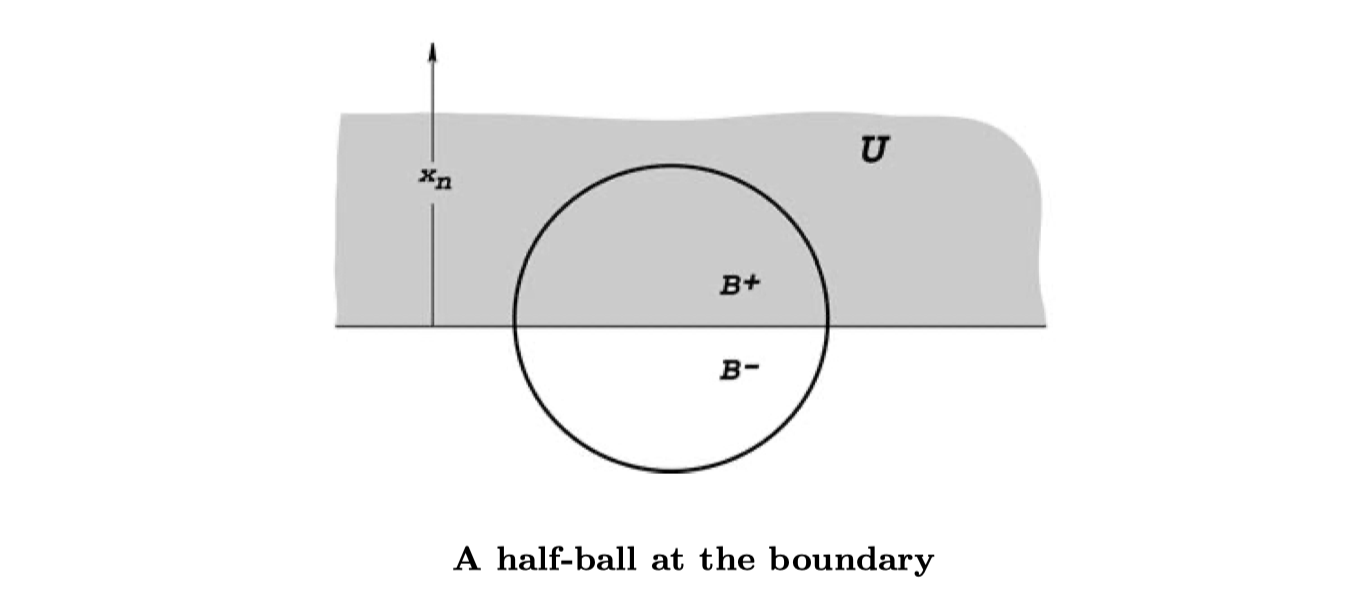
\includegraphics[width=0.8\textwidth]{figures/half-ball-boundary.png}
\end{figure}
$$
\begin{aligned}
\int_{\Gamma}|u|^{p} d x^{\prime} & \leq \int_{\left\{x_{n}=0\right\}} \zeta|u|^{p} d x^{\prime}=-\int_{B^{+}}\left(\zeta|u|^{p}\right)_{x_{n}} d x \\
&=-\int_{B^{+}}|u|^{p} \zeta_{x_{n}}+p|u|^{p-1}(\operatorname{sgn} u) u_{x_{n}} \zeta d x \\
& \leq C \int_{B^{+}}|u|^{p}+|D u|^{p} d x
\end{aligned}
$$
where we employed Young's inequality.
\begin{figure}[H]
    \centering
    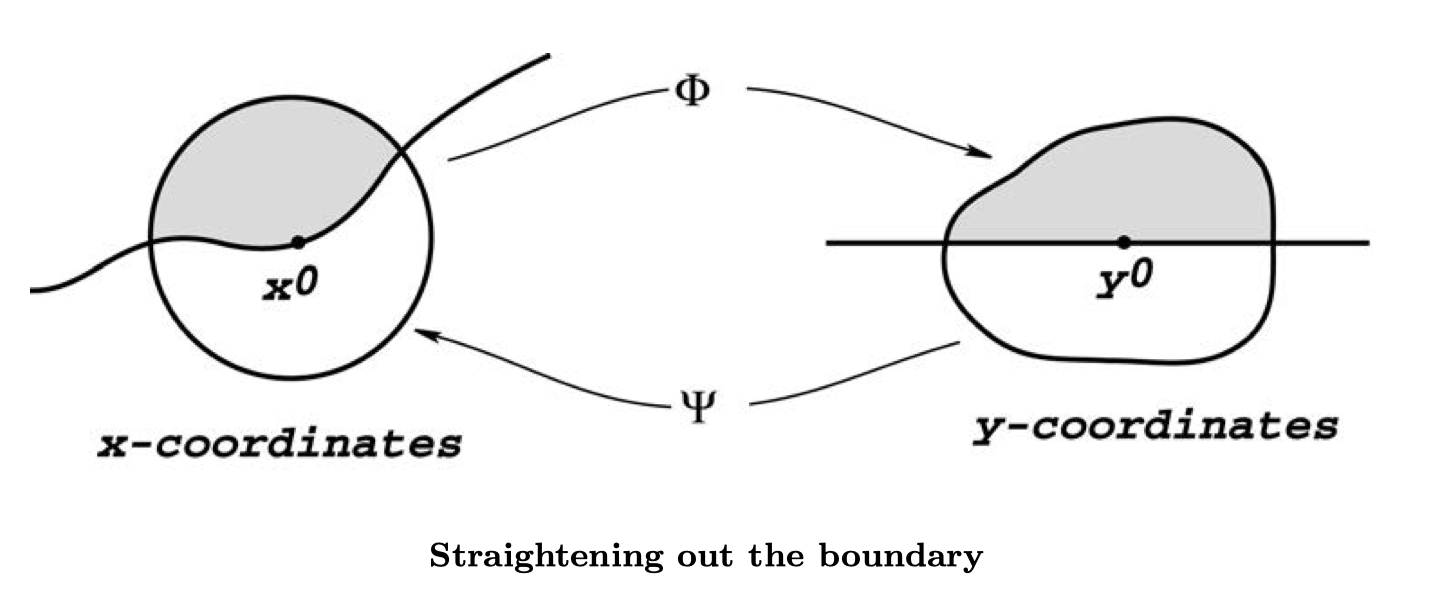
\includegraphics[width=0.8\textwidth]{figures/Straightening-boundary.png}
\end{figure}
\end{proof}

\begin{remark}
The map $tr_{\partial u}: W^{1,p}(U) \to L^p(\partial  U)$ is not surjective.
\end{remark}

Now, we will understand the sharp trace theorem in a restricted setting.

The setting we have in mind is $p=2$. The advantage here is that we may use the theory of the Fourier transform and Plancherel's theorem. We will also focus on the domain $U=\mathbb{R}_{+}^{d}=\left\{x \in \mathbb{R}^{d}: x^{d}>0\right\}$ with boundary $\left\{\left(x^{\prime}, 0\right) \in \mathbb{R}^{d}\right\} \cong \mathbb{R}^{d-1}$, where $x^{\prime}:=\left(x^{1}, \ldots, x^{d-1}\right)$.
Recall the Fourier transform characterization of the $H^{k}$ norm:
$$
\|u\|_{H^{k}}^{2} \simeq\left\|\left(1+|\xi|^{2}\right)^{k / 2} \widehat{u}\right\|_{L_{\xi}^{2}}^{2}, \quad k \geq 0 \text { an integer. }
$$
If we replace $k$ with any $s \in \mathbb{R}$, we can talk about \textbf{fractional ( $L^{2}$-based) Sobolev spaces}.

\begin{definition}
[Fractional Sobolev spaces]
The space of distributions equipped with the norm 
\[
    \|u\|_{H^{k}}^{2} \simeq\left\|\left(1+|\xi|^{2}\right)^{k / 2} \widehat{u}\right\|_{L_{\xi}^{2}}^{2},
\]
where $k$ is any real number.
\end{definition}

\begin{theorem}
[Sharp trace theorem]
For $u \in C^{1}\left(\overline{\mathbb{R}_{+}^{d}}\right) \cap H^{1}\left(\mathbb{R}_{+}^{d}\right)$,
$$
\left\|\operatorname{tr}_{\partial U} u\right\|_{H^{1 / 2}\left(\mathbb{R}^{d-1}\right)} \leq C\|u\|_{H^{1}\left(\mathbb{R}_{+}^{d}\right)} .
$$
\end{theorem}
\begin{proof}
    Proof. Take $u \in C^{1}\left(\overline{\mathbb{R}_{+}^{d}}\right) \cap H^{1}\left(\mathbb{R}_{+}^{d}\right)$. Using the extension procedure from last time, we can find a $\tilde{u} \in C^{1}\left(\mathbb{R}^{d}\right)$ such that
$$
\|\tilde{u}\|_{H^{1}\left(\mathbb{R}^{d}\right)} \leq C\|u\|_{H^{1}\left(\mathbb{R}_{+}^{d}\right)}
$$
Then
$$
\begin{aligned}
\operatorname{tr}_{\partial U} u\left(x^{\prime}\right) &=u\left(x^{\prime}, 0\right) \\
&=\widetilde{u}\left(x^{\prime}, 0\right) \\
&=\int \mathcal{F}_{x^{d}} \widetilde{u}\left(x^{\prime}, \xi_{d}\right) \frac{1}{2 \pi} d \xi_{d}
\end{aligned}
$$
On the other hand,
$$
\mathcal{F}_{x^{\prime},0} \operatorname{tr}_{\partial U} u\left(\xi^{\prime}\right)=\int \mathcal{F} \widetilde{u}\left(\xi^{\prime}, \xi_{d}\right) \frac{1}{2 \pi} d \xi_{d}
$$
For now, let us not assume $s=1 / 2$ so we can see where this choice comes from.
$$
\begin{aligned}
\|\operatorname{tr} \partial U u\|_{H^{s}\left(\mathbb{R}^{d-1}\right)} & \sim\left\|\left(1+\left|\xi^{\prime}\right|^{2}\right)^{s / 2} \mathcal{F}_{x^{\prime}} \operatorname{tr} u\left(\xi^{\prime},0\right)\right\|_{L_{\xi^{\prime}}^{2}} \\
&=\left\|\left(1+\left|\xi^{\prime}\right|^{2}\right)^{s / 2} \int \mathcal{F} \widetilde{u}\left(\xi^{\prime}, \xi_{d}\right) \frac{1}{2 \pi} d \xi_{d}\right\|_{L_{\xi^{\prime}}^{2}} \\
\text { Writing }|\xi|^{2}=\left|\xi^{\prime}\right|^{2}+& \xi_{d}^{2}, \\
&=\left\|\int \frac{\left(1+\left|\xi^{\prime}\right|^{2}\right)^{s / 2}}{\left(1+\left|\xi^{\prime}\right|^{2}+\xi_{d}^{2}\right)^{1 / 2}}\left(\left(1+\left|\xi^{\prime}\right|^{2}+\xi_{d}^{2}\right)^{1 / 2} \mathcal{F} \widetilde{u}\right) \frac{1}{2 \pi} d \xi_{d}\right\|_{L_{\xi^{\prime}}^{2}}
\end{aligned}
$$
Applying Cauchy-Schwarz,
$$
\begin{aligned}
&\leq\left\|\left(\int \frac{\left(1+\left|\xi^{\prime}\right|^{2}\right)^{s}}{1+\left|\xi^{\prime}\right|^{2}+\xi_{d}^{2}} d \xi_{d}\right)^{1 / 2}\left\|\left(1+\left.|\xi|^{\prime}\right|^{2}+\xi_{d}^{2}\right)^{1 / 2} \mathcal{F} \widetilde{u}\right\|_{L_{\xi_{d}}^{2}}\right\|_{L_{\xi^{\prime}}^{2}} \\
&\leq \sup _{\xi^{\prime} \in \mathbb{R}^{d-1}}\left(\int \frac{\left(1+\left|\xi^{\prime}\right|^{2}\right)^{s}}{1+\left|\xi^{\prime}\right|^{2}+\xi_{d}^{2}} d \xi_{d}\right)^{1 / 2} \underbrace{\left \|\left\|\left(1+\left.|\xi|^{\prime}\right|^{2}+\xi_{d}^{2}\right)^{1 / 2} \mathcal{F} \widetilde{u}\right\|_{L_{\xi_{d}}^{2}} \right\|_{L_{\xi}^{2}}}_{\|u\|_{H^{1}}}
\end{aligned}
$$
For what $s$ is this supremum $<+\infty$ ? This is $s \leq 1 / 2$.
\qed
\end{proof}

In fact, it turns out that the image of $\tr_{\partial U}$ is exactly $H^{\frac{1}{2}}$. 

\begin{theorem}
[Extension from $\partial U$] 
There exists a bounded linear map
$$
\operatorname{ext}_{\partial U}: H^{1 / 2}\left(\mathbb{R}^{d-1}\right) \rightarrow H^{1}\left(\mathbb{R}_{+}^{d}\right)
$$
such that $\operatorname{tr}_{\partial U} \circ \operatorname{ext}_{\partial U}=\mathrm{id}$.
\end{theorem}
\begin{proof}
We will use the Poisson semigroup. Suppose we are given $g \in \mathcal{S}\left(\mathbb{R}^{d-1}\right)$, and let $\eta \in C_{c}^{\infty}(\mathbb{R})$ be such that $\eta=1$ for $|s|<1$ and $\eta=0$ for $|s|>2$. Define $u=$ ext $_{\partial U} g$ by
$$
\mathcal{F}_{x^{\prime}} u\left(\xi^{\prime}, x^{d}\right)=\eta\left(x^{d}\right) e^{-x^{d}\left|\xi^{\prime}\right|} \widehat{g}(\xi)
$$
This right term is the solution to the Laplace equation on the half-space with boundary data $g$.
We need to show that
$$
u \in H^{1}\left(\mathbb{R}_{+}^{d}\right) \Longleftrightarrow(\mathrm{i}) u, \partial_{1} u, \ldots, \partial_{d-1} u \in L^{2}
$$
(ii) $\partial_{d} u \in L^{2}$.
(i) implies:
$$
\begin{aligned}
\|u\|_{L^{2}}^{2}+\left\|\partial_{1} u\right\|_{L^{2}}^{2}+\cdots+\left\|\partial_{d-1} u\right\|_{L^{2}}^{2} &=\left\|\left(1+\left|\xi^{\prime}\right|^{2}\right)^{1 / 2} \mathcal{F}_{x^{\prime}} u\left(\xi^{\prime}, x^{d}\right)\right\|_{L^{\prime}}^{2} L_{x^{d}} \\
&=\|\left(1+\left|\xi^{\prime}\right|^{2}\right)^{1 / 2} \eta\left(x^{d}\right) e^{-x^{d}\left|\xi^{\prime}\right| } \widehat{g}\left(\xi^{\prime}\right) \|_{L_{\xi^{\prime}}^{2} L_{x^{d}}^{2}}^{2}
\end{aligned}
$$
We can integrate in any order, so integrate the $x^{d}$ integral first.
$$
=\|\underbrace{\left(1+\left|\xi^{\prime}\right|^{2}\right)^{1 / 4}\left\|\eta\left(x^{d}\right) e^{-x^{d}\left|\xi^{\prime}\right|}\right\|_{L_{x d}^{2}}}_{\text {NTS this is unif. bdd. } \xi^{\prime} \in \mathbb{R}^{d-1}}\left(1+\left|\xi^{\prime}\right|^{2}\right)^{1 / 4} \widehat{g}\left(\xi^{\prime}\right)\|_{L_{\xi^{\prime}}^{2}}^{2}
$$
We can use the bound
$$
\left\|\eta\left(x^{d}\right) e^{-x^{d}\left|\xi^{\prime}\right|}\right\|_{L_{x^{d}}^{2}}^{2} \lesssim 1
$$
and the substitution bound
$$
\int \eta^{2}\left(x^{d}\right) e^{-2 x^{d}\left|\xi^{\prime}\right|} d x^{d} \lesssim \frac{1}{\left|\xi^{\prime}\right|}
$$
This gives
$$
\left\|\eta\left(x^{d}\right) e^{-x^{d}\left|\xi^{\prime}\right|}\right\|_{L_{x^{d}}^{2}} \lesssim \min \left\{1, \frac{1}{\left|\xi^{\prime}\right|^{1 / 2}}\right\} \lesssim\left(1+\left|\xi^{\prime}\right|^2\right)^{-1 / 4}
$$
Hence,
\[
    \|u\|_{L^{2}}^{2}+\left\|\partial_{1} u\right\|_{L^{2}}^{2}+\cdots+\left\|\partial_{d-1} u\right\|_{L^{2}}^{2} \le \|(1+|\xi'|^2)^{1/4} \hat g(\xi')\|^2_{L_{\xi'}^2} = \|g\|_{H^{1/2}}^2.
\]
(ii) implies:
$$
\begin{aligned}
\partial_{x^{d}} u &=\partial_{x^{d}}\left(\eta\left(x^{d}\right) v\right), \quad \mathcal{F}_{x^{\prime}} v=e^{-x^{d}\left|\xi^{\prime}\right|} \widehat{g}(\xi) \\
&=\eta^{\prime}\left(x^{d}\right) v+\eta \partial_{x^{d}} v
\end{aligned}
$$
The norm of the first term is bounded by $\|v\|_{L^{2}\left(x^{d} \in \operatorname{supp} \eta\right)}$, and the norm of the second term is
$$
\begin{aligned}
\left\|\eta \partial_{x^{d}} v\right\|_{L_{x^{\prime}}^{2} L_{\xi_{d}}^{2}} &=\left\|\eta \partial_{x^{d}}\left(e^{-x^{d}\left|\xi^{\prime}\right|} \widehat{g}\left(\xi^{\prime}\right)\right)\right\|_{L_{\xi^{\prime}}^{2} L_{x^{d}}^{2}} \\
&=\|\left|\xi^{\prime}\right| \underbrace{e^{-x^{d} \mid \xi^{\prime}} \mid \widehat{g}\left(\xi^{\prime}\right) \eta\left(x^{d}\right)}_{\mathcal{F}_{x^{\prime}} u}\|_{L_{\xi^{\prime}}^{2} L_{x^{d}}^{2}}
\end{aligned}
$$
We can use tricks in (i) again, 
$$
\left\|\eta \partial_{x^{d}} v\right\|_{L_{x^{\prime}}^{2} L_{\xi_{d}}^{2}}\leq C\|g\|_{H^{1 / 2} .}
$$
\qed
\end{proof}
\begin{remark}
\begin{itemize}
    \item []
    \item In fact, by the usual smooth partition of unity argument with boundary straightening, one can define $H^{1 / 2}(\partial U)$ for $\partial U$ of class $C^{1}$ and prove the sharp trace theorem. The independence of this space from the smooth partition of unity and boundary straightening follows from interpolation theory (which you can find in the 1970 textbook of Stein).
    \item For $p \neq 2, \operatorname{im}\left(\operatorname{tr}_{\partial U} W^{1, p}(U)\right)=B_{p}^{1-1 / p, p}(\partial U)$. This is called the $L^{p}-$ Besov space of order $1-1 / p$ and summability index $p$. This is also covered in Stein's book.
\end{itemize}
\end{remark}


%%%%%%%%%%%%% 
% Sobolev Inequality 
\newpage
\section{Sobolev Inequalities}
Sobolev-type inequalities are quantitative generations of fundamental theorem of calculus, 
which use derivatives to control function. Below we will prove them for smooth functions, and 
then according to density theorems, these inequalities hold in the corresponding Sobolev spaces.

\begin{theorem}
[Gaglierdo-Nirenberg-Sobolev  inequality]
Let $d \geq 2$. For $u \in C_{c}^{\infty}\left(\mathbb{R}^{d}\right)$, we have
$$
\|u\|_{L^{\frac{d}{d-1}}\left(\mathbb{R}^{d}\right)} \leq C_{d}\|D u\|_{L^{1}\left(\mathbb{R}^{d}\right)},
$$
where $C_{d}$ is a constant depending only on $d$.
\end{theorem}

\begin{remark}
    The exponent on the left hand side need not be remembered because it can be derived from scaling considerations (dimensional analysis). In particular, first observe that both sides are homogeneous: if $u \mapsto u_{\lambda}(x)=u(x / \lambda)$ for $\lambda>0$, then
    $$
    \begin{aligned}
    \left\|u_{\lambda}\right\|_{L^{p}} &=(\lambda^{d} \underbrace{\int\left|u\left(\frac{x}{\lambda}\right)\right|^{p} \frac{1}{\lambda^{d}} d x}_{=\int|u|^{p} d x^{\prime}})^{1 / p} \\
    &=\lambda^{d / p}\|u\|_{L^{p}}
    \end{aligned}
    $$
    On the other hand, $D\left(u_{\lambda}\right)=\frac{1}{\lambda}(D u)_{\lambda}$, so
    $$
    \left\|D\left(u_{\lambda}\right)\right\|_{L^{p}}=\frac{1}{\lambda} \lambda^{d / p}\|D u\|_{L^{p}}
    $$
    Now compare these:
    $$
    \begin{aligned}
    \left\|u_{\lambda}\right\|_{L^{p}} \leq c\left\|D u_{\lambda}\right\|_{L^{1}} \quad \forall \lambda>0 & \Longleftrightarrow \lambda^{d / p}\|u\|_{L^{p}} \leq c \lambda^{-1+d}\|D u\|_{L^{1}} \quad \forall \lambda>0 \\
    & \Longleftrightarrow \frac{d}{p}=d-1 \\
    & \Longleftrightarrow p=\frac{d}{d-1} .
    \end{aligned}
    $$
\end{remark}
All we are doing here is changing the unit of length and requiring that the inequality is invariant under our unit of length.

To prove this theorem, the key ingredient is another inequality. Denoting $\left(x^{1}, \ldots, \widehat{x}^{j}, \cdots, x^{d}\right)=\left(x^{1}, \ldots, x^{j-1}, x^{j+1}, \ldots, x^{d}\right)$, we have the following.

\begin{lemma}
    [Loomis-Whitney inequality]. Let $d \geq 2$. For $j=1, \ldots, d$, suppose $f_{j}=$ $f_{j}\left(x^{1}, \ldots, \widehat{x}^{j}, \ldots, x^{d}\right)$. Then
    $$
    \left\|\prod_{j=1}^{d} f_{j}\right\|_{L^{1}\left(\mathbb{R}^{d}\right)} \leq \prod_{j=1}^{d}\left\|f_{j}\right\|_{L^{d-1}\left(\mathbb{R}^{d-1}\right)}
    $$

\end{lemma}
\begin{proof}
     Integrate in each variable and apply Hölder:
    $$
    \begin{aligned}
    \int\left|\prod_{j=1}^{d} f_{j}\right| d x^{1} &=\left|f_{1}\right| \int\left|f_{2}\right| \cdots\left|f_{d}\right| d x^{1} \\
    & \leq\left|f_{1}\right|\left\|f_{2}\right\|_{L_{x^{1}}^{d-1}} \cdots\left\|f_{d}\right\|_{L_{x^{1}}^{d-1}}
    \end{aligned}
    $$
    This is a function of $\left(x^{2}, \ldots, x^{d}\right)$. Now integrate with respect to the next variable:
$$
\begin{aligned}
\iint\left|\prod_{j=1}^{d} f_{j}\right| d x^{1} d x^{2} & \leq \int\left|f_{1}\right|\left\|f_{2}\right\|_{L_{x^{1}}^{d-1}} \cdots\left\|f_{d}\right\|_{L_{x^{1}}^{d-1}} d x^{2} \\
&=\left\|f_{2}\right\|_{L_{x^{1}}^{d-1}}\left\|f_{1}\right\|_{L_{x^{2}}^{d-1}}\left\|f_{3}\right\|_{L_{x^{1}, x^{2}}^{d-1}} \cdots\left\|f_{d}\right\|_{L_{x^{1}, x^{2}}^{d-1}}
\end{aligned}
$$
Iterating this gives the inequality.
\qed 
\end{proof}


\begin{remark}
    The Loomis-Whitney inequality answers the following geometric question. Suppose $E \subseteq \mathbb{R}^{d}$, and know the projections $\pi_{j}(E)$. Can we bound the measure of $E$ by $\left|\pi_{j}(E)\right|$ ?
    \begin{figure}[H]
        \centering
         \incfig[0.7]{1-Loomis}
    \end{figure}
    Yes!
$$
\begin{aligned}
|E| &=\int \one_{E} d x \\
& \leq \int \prod_{j=1}^{d} \one_{\pi_{j}(E)}\left(x^{1}, \ldots, \widehat{x}^{j}, \ldots, x^{d}\right) d x \\
& \stackrel{\mathrm{L}-\mathrm{W}}{\leq} \prod_{j=1}^{d}\left|\pi_{j}(E)\right|^{\frac{1}{d-1}} .
\end{aligned}
$$
\end{remark}

Now let's prove the GNS inequality. 
\vspace{2em}
\begin{proof}[][Proof of GNS inequality]
 Observe that if we take a point $x \in \mathbb{R}^{d}$, then we can write
$$
u(x)=\int_{-\infty}^{x^{j}} \partial_{x^{j}} u\left(x^{1}, \ldots, x^{j-1}, y, x^{j+1}, \ldots, x^{d}\right) d y,
$$
using the fundamental theorem of calculus. Here, we use the compact support assumption to be sure this converges. This means that
$$
|u(x)| \leq \int_{-\infty}^{x^{j}}\left|\partial_{x^{j}} u\left(x^{1}, \ldots, x^{j-1}, y, x^{j+1}, \ldots, x^{d}\right)\right| d y .
$$
We can upper bound this by replacing $x^{j}$ by $\infty$ and $\partial_{x^{j}}$ by $D$ :
$$
|u(x)| \leq \underbrace{\int_{-\infty}^{\infty}\left|D u\left(x^{1}, \ldots, x^{j-1}, y, x^{j+1}, \ldots, x^{d}\right)\right| d y}_{\tilde{f}_{j}\left(x^{1}, \ldots, \widehat{x}^{j}, \ldots, x^{d}\right)} .
$$
This means that we have
$$
|u(x)|^d \leq\left(\prod_{j=1}^{d} \widetilde{f}_{j}\right)
$$
which we can write as
$$
|u(x)|^{\frac{d}{d-1}} \leq\left(\prod_{j=1}^{d} \widetilde{f}_{j}^{\frac{1}{d-1}}\right),
$$
Using the Loomis-Whitney inequality and let $ f_j = \tilde f_j^{\frac{1}{d-1}} $,
$$ 
\begin{aligned}
\|u\|_{L^{\frac{d}{d-1}}}^{\frac{d}{d-1}} &=\int|u|^{\frac{d}{d-1}} d x \\
& \leq \int \prod_{j=1}^{d} f_{j} d x \\
& \leq \prod_{j=1}^{d}\left\|f_{j}\right\|_{L^{d-1}} \\
&=\prod_{j=1}^{d}\left(\int\left|f_{j}\right|^{d-1} d x^{1} \cdots \widehat{d x^{j}} \cdots d x^{d}\right)^{\frac{1}{d-1}}
\end{aligned}
$$
Observe that $\left|f_{j}\right|^{d-1}=\int_{-\infty}^{\infty}\left|D u\left(x^{1}, \ldots, x^{j}, \ldots, x^{d}\right)\right| d x^{j}$, so
$$
\leq\|D u\|_{L^{1}}^{\frac{d}{d-1}} .
$$
\qed
\end{proof}
\begin{remark}
    GNS is the functional counterpart of the isoperimetric inequality. Given a function, we can make a layer cake decomposition in the $y$ axis and apply the isoperimetric inequality to each part. This is useful for functions on manifolds where we have some geometric information.
\end{remark}

\subsection{Sobolev inequalities with $p<d$}
Now we will upgrade this to the case where we have other $L^{p}$ spaces on the right hand side.
\begin{theorem}
    [Sobolev inequalities for $L^{p}$-based spaces] Let $d \geq 2$, and assume that $1<p<d$. For $u \in C_{c}^{\infty}\left(\mathbb{R}^{d}\right)$, we have
    $$
    \|u\|_{L^{q}\left(\mathbb{R}^{d}\right) }\leq C\|D u\|_{L^{p}\left(\mathbb{R}^{d}\right)}
    $$
    where $q=\frac{d p}{d-p}$.
\end{theorem}
What is $q$ ? We do dimensional analysis to figure out the exponent. On the left hand side, we have $[x]^{d / q}$, and on the right hand side, we have $[x]^{-1+d / p}$. If we solve for $q$, we get $q=\frac{d p}{d-p}$. This also gives us the restriction that $p<d$.

\vspace{2em}
\begin{proof}
    Take $v=\left|u\right|^{\widetilde{q}}$, where $\widetilde{q}=\frac{q}{d /(d-1)}$. Its derivative is $|D v|=\tilde q|u|^{\tilde q-1}|D v|$. This can be justified using approximation: approximate $|x|$ by $\left(\varepsilon^{2}+x^{2}\right)^{1 / 2} \mathrm{v}$ and let $\varepsilon \rightarrow 0$. Then
    $$
    \int|u|^{q} d x=\int|v|^{\frac{d}{d-1}} d x
    $$
    Using the GNS inequality,
    $$
    \leq\left(\int|D v| d x\right)^{\frac{d-1}{d}}
    $$
    It is at this point that we need the above approximation. But it works, using the dominated convergence theorem.
    $$
    =\left(\int|u|^{\widetilde{q}-1}|D u| d x\right)^{\frac{d-1}{d}}
    $$
    Using H\"older's inequality, we can put $|D u|$ into $L^{p}$, which puts $|u|^{\tilde q-1}$ in $L^{p^{\prime}}$. By dimensional analysis, it must happen that
    $$
\leq (\int |u| ^{(\tilde q-1)\frac{p}{p-1}} dx )^{\frac{(p-1)(d-1)}{pd}}  \|D u\|_{L^{p}}^{\frac{d-1}{d}} = \|u\|_{L^q}^{q - \frac{d-1}{d}} \|Du \|_{L^{p}}^{\frac{d-1}{d}}.
$$
This completes the proof.
\qed 
\end{proof}
Now we will upgrade this to every element in the abstract Sobolev space and to situations where we have a function which is bounded on an abstract domain.

\begin{theorem}
    Let $d \geq 2$, and assume that $1 \leq p<d$.
    \begin{itemize}
        \item (i) For $u \in W^{1, p}\left(\mathbb{R}^{d}\right)$,
        $$
        \|u\|_{L^{q}\left(\mathbb{R}^{d}\right)} \leq C\|D u\|_{L^{p}\left(\mathbb{R}^{d}\right)},
        $$
        where $q=\frac{d p}{d-p}$.

        \item Let $U$ be a bounded domain with $C^{1}$ boundary $\partial U$. Then for $u \in W^{1, p}(U)$,
        $$
        \|u\|_{L^{q}(U)} \leq C\| u\|_{W^{1, p}(U)}
        $$
        where $q=\frac{d p}{d-p}$.
    \end{itemize}
\end{theorem}
\begin{proof}
     For the first part, we can use density theorem of $C_{c}^{\infty}$ in $W^{1, p}\left(\mathbb{R}^{d}\right)$. For the second theorem, we need to first use extension theorem then use density theorem. Note that G-N-S inequality only works for $C_{c}^{\infty}$ functions.
     \qed 
\end{proof}

We have another further result for $W_0^{1,p}(U)$:
\begin{theorem}
[Estimates for $W_0^{1,p}(U)$] For $1\leq p<d$ (which makes $d\geq 2$), $U$ is a bounded domain. For $u\in W_0^{1,p}(U)$, we have
$$\|u\|_{L^q(U)}\leq C\|Du\|_{L^p(U)},\quad \forall 1\leq q\leq p^*$$
\end{theorem}
Note that the difference from the previous theorem is that the right hand side is $\|Du\|_{L^p(U)}$ instead of $\|u\|_{W^{1,p}(U)}$. The proof of this theorem requires the approximation of $C_c^{\infty}$ directly, without extension.
Particularly,  we have
$$
\|u\|_{L^p(U)}\leq C\|Du\|_{L^p(U)}
$$
This is called \textbf{Poincare-Fredrich inequality}, one of the \textbf{Poincare-type inequalities}.

\subsection{Sobolev Inequalities with $p>d$}
Next, we investigate: What does $\|u\|_{W^{1, p}}$ tell us when $p \geq d$ ? This will be based on another way to relate $u$ with its derivative, $D u$. Start with $u \in C^{\infty}\left(\mathbb{R}^{d}\right)$, and write down what we get by applying the fundamental theorem of calculus:
$$
u(x)-u(y)=\int_{0}^{1} \frac{d}{d s} u(x+s(y-x)) d s .
$$
The key idea is to average to take advantage of the fact that we are in multiple dimensions. Take absolute values and average this in $y$ : Fix $r>0$, so
$$
\frac{1}{\left|B_{r}(x)\right|} \int_{B_{r}}|u(x)-u(y)| d y \leq \frac{1}{\left|B_{r}(x)\right|} \int_{B_{r}(x)} \int_{0}^{1}\left|\frac{d}{d s} u(x+s(y-x))\right| d s d y
$$
By the chain rule, this derivative is $(y-x) \cdot D u(x+s(y-x))$.
$$
\leq C \frac{1}{r^{d}} \int_{B_{r}(x)} \int_{0}^{1}|x-y \| D u(x+s(y-x))| d s d y
$$
Let $\rho \omega=y-x$, so that $\rho=|y-x|$.
$$
=C \frac{1}{r^{d}} \int_{0}^{r} \int_{\mathbb{S}^{d-1}} \int_{0}^{1} \rho|D u(x+s \rho \omega)| d s \rho^{d-1} d \omega d \rho
$$
Make another change of variables, so we can make $x+s \rho \omega$ into an actual radius and then evaluate on of the integrals. We do $t=s \rho$
$$
=C \frac{1}{r^{d}} \int_{0}^{r} \int_{\mathbb{S}^{d-1}} \int_{0}^{1} \frac{t^{d}}{s^{d}} \frac{1}{s}|D u(x+t \omega)| d s d \omega d t
$$
Simplify the $s$ integral and upper bound $t \leq r$ :
$$
\begin{aligned}
&\leq C \int_{0}^{r} \int_{\mathbb{S}^{d-1}}|D u(x+t \omega)| d \omega d t \\
&=C \int_{B_{r}(x)} \frac{|D u|}{|x-y|^{d-1}} d y
\end{aligned}
$$

We can summarize this as a lemma: 
\begin{lemma}
    \label{lem: ball-ineq}
    Let $p>d$, let $d \geq 2$, and let $u \in C^{\infty}\left(\mathbb{R}^{d}\right)$. Then
    $$
    \frac{1}{\left|B_{r}(x)\right|} \int_{B_{r}}|u(x)-u(y)| d y \leq C \int_{B_{r}(x)} \frac{|D u|}{|x-y|^{d-1}} d y
    $$

\end{lemma}

\begin{theorem}
[Sobolev ineq, $p>d$]
Let $p>d$ with $d \geq 2$, and take $u \in C^{\infty}\left(\mathbb{R}^{d}\right)$. Then
$$
|u(x)-u(y)| \leq C|x-y|^{\alpha}\|D u\|_{L^{p}\left(\mathbb{R}^{d}\right)},
$$
where $\alpha=1-\frac{d}{p}$.
\end{theorem}
\begin{proof}
    We will use the lemma. The idea is to introduce an auxiliary variable $z$ and take the average over $z$ on some domain $U$ :
    $\frac{1}{|U|} \int_{U}|u(x)-u(y)| d z \leq \frac{1}{|U|} \int_{U}|u(x)-u(z)| d z+\frac{1}{|U|} \int_{U}|u(y)-u(y)| d z$
    Since $\frac{\left|B_{r}(x)\right|}{|U|} \simeq 1$,
    $$
    \begin{aligned}
    &\lesssim \frac{\left|B_{r}(x)\right|}{|U|} \int_{B_{r}(x)}|u(x)-u(z)| d z+\frac{\left|B_{r}(y)\right|}{|U|} \int_{B_{r}(y)}|u(y)-u(z)| d z \\
    &\lesssim \int_{B_{r}(x)} \frac{|D u|}{|x-z|^{d-1}} d z+\int_{B_{r}(y)} \frac{|D u|}{|y-z|^{d-1}} d z \\
    &\lesssim\|D u\|_{L^{p}}\left\|\frac{1}{|x-z|^{d-1}}\right\|_{L^{p^{\prime}}\left(B_{r}(x)\right)}+\|D u\|_{L^{p}}\left\|\frac{1}{|y-z|^{d-1}}\right\|_{L^{p^{\prime}}\left(B_{r}(y)\right)}
    \end{aligned}
    $$
    Now we just need to evaluate
    $$
    \int_{B_{r}(0)} \frac{1}{|z|^{(d-1) p^{\prime}}} d z \simeq r^{\alpha p'}
    $$
    \qed 
\end{proof}

 \begin{remark}
    Again, we can find the value of $\alpha$ by dimensional analysis: $1=\alpha+(-1)+\frac{d}{p}$ gives $\alpha=1-\frac{d}{p}$.
 \end{remark}
 We want to rephrase this as an inequality for $u \in W^{1, p}(U)$. To do this, we need a space that has a regularity property relating to the theorem above.

 \begin{definition}
 [H\"older seminorm]
Let $u \in C(I)$. The Hölder seminorm of order $\alpha$ is
$$
[u]_{C^{\alpha}(U)}=\sup _{x \neq y} \frac{|u(x)-u(y)|}{|x-y|^{\alpha}} .
$$
 \end{definition}
 By a \textbf{seminorm}, we mean that $[\cdot]_{C^{\alpha}(U)}$ satisfies all the properties of a norm except the property that $[u]_{C^{\alpha}(U)}=0 \Longrightarrow u=0$. Instead, this implies that $u$ is constant. Here is how we make it into a norm\dots
 
 \begin{definition}
 [H\"older norm \& H\"older space]
The H\"older norm of order $\alpha$ is
$$
\|u\|_{C^{\alpha}(U)}=[u]_{C^{\alpha}(U)}+\|u\|_{L^{\infty}} .
$$
The H\"older space of order $\alpha$ is
$$
C^{0,\alpha}(U)=\left\{u \in C(U):\|u\|_{C^{\alpha}}<\infty\right\} .
$$
This definition could be generalized to define Holder space $C^{k, \alpha}$ :
$$
C^{k, \alpha}(U)=\left\{u \in C^{k}(U),\left\|D^{\beta} u\right\|_{C^{0, \alpha}}<\infty, \forall \beta,|\beta|=k\right\}
$$
and 
\[
    \|u\|_{C^{k,\alpha}(U)} = \sum_{|\alpha| \le k} \|D^\alpha u\|_{L^\infty} + \sum_{|\alpha|=k} [D^\alpha u]_{C^{0,\alpha}(U)}.
\]
 \end{definition}

 \begin{theorem}
    [Morrey's inequality] Let $d \geq 2$, let $p>d$, and let $U$ be a bounded domain in $\mathbb{R}^{d}$ with $C^{1}$ boundary $\partial U$ \footnote{This is sometimes called Morey's embedding}. If $u \in W^{1, p}(U)$, then $u \in C^{\alpha}(U)$ with $\alpha=1-\frac{d}{p}$. Moreover,
    $$
    \|u\|_{C^{0,\alpha}(U)} \leq C\|u\|_{W^{1, p}(U)} .
    $$
 \end{theorem}
 \begin{proof}
    By extension and density theorems, it suffices to consider $u \in C^{\infty}\left(\mathbb{R}^{d}\right)$ with supp $u \subseteq$ $V$, where $V$ is a bounded, open set with $V \supseteq \bar{U}$ (chosen independently of $u$ ). By the previous theorem,
    $$
    [u]_{C^{\alpha}(V)} \leq C\|u\|_{W^{1, p}} .
    $$
    So all that remains is to bound $\|u\|_{L^{\infty}}$ in terms of $\|u\|_{W^{1, p}}$. For this purpose, we will again use the lemma to approximate $u$ by its average. Let $x \in V$, then
    \[
        \begin{aligned}
            \left|u(x)-\frac{1}{\left|B_{r}(x)\right|} \int_{B_{r}(x)} u d z\right| & \leq\left|\frac{1}{\left|B_{r}(x)\right|} \int_{B_{r}(x)} u(x)-u(z) d z\right| \\
            & \leq \frac{1}{\left|B_{r}(x)\right|} \int_{B_{r}(x)}|u(x)-u(z)| d z \\
            & \leq C \int_{B_{r}(x)} \frac{|D u(z)|}{|z-x|^{d-1}} d z \\
            & \leq C r^{\alpha}\|D u\|_{L^{p}\left(B_{r}(x)\right)} .
            \end{aligned}
    \]
    Take $r=1$, then 
    \[
        \begin{aligned}
            &|u(x)| \leq C \underbrace{\left|\int_{B_{r}(x)} u d z\right| d z }_{\leq \int_{B_1(x)}|u|\,dz\leq C\|u\|_{L^p(B_1(0))}}+C\|D u\|_{L^p}\\
            &\leq C\left(\|u\|_{L^{p}}+\|D u\|_{L^{p}}\right) \text {. }
            \end{aligned}
    \]
    \qed 
 \end{proof}

 \subsection{Sobolev Inequalities with $p=d$}

 What about when $p=d$ (and $d \geq 2)$ ? In this case, the inequality $\|u\|_{L^{\infty}(U)} \leq\|u\|_{W^{1, d}(U)}$ fails.
 
 \begin{example}
    Here is a counterexample to the above inequality when $p=d=2$. Take $U=B_{1}(0) \subseteq \mathbb{R}^{2}$ and
    $$
    u(x)=\log \log \left(10+\frac{1}{|x|}\right) \text {. }
    $$
 
 \end{example}

 A popular remedy for $p=d$ is to think about bounded mean oscillation:

 \begin{definition}
 [BMO seminorm]
Let $u \in L_{\mathrm{loc}}^{1}(U)$. The BMO seminorm is
 $$
 [u]_{\mathrm{BMO}}=\sup _{B_{r}\left(x_{0}\right) \subseteq U} \frac{1}{\left|B_{r}\left(x_{0}\right)\right|} \int_{B_{r}\left(x_{0}\right)}\left|u(z)-\frac{1}{\left|B_{r}\left(x_{0}\right)\right|} \int_{B_{r}\left(x_{0}\right)} u\right| d z .
 $$
 \end{definition}

 Recall that we have Hardy-Littlewood theorem. 
\begin{theorem}
[Hardy-Littlewood]
\label{thm:Hardy-Littlewood}
Let $u \in L_{\mathrm{loc}}^{1}$, and define
$$
\mathcal{M} u(x)=\sup _{r>0} \frac{1}{\left|B_{r}(x)\right|} \int_{B_{r}(x)}|u| .
$$
(Note that $\left.|\mathcal{M} u| \leq\|u\|_{L^{\infty}}\right)$. For $1<p \leq \infty$,
$$
\|\mathcal{M} u\|_{L^{p}} \leq C\|u\|_{L^{p}} .
$$
\end{theorem}
 
 We have the following theorem: 

\begin{theorem}
    \label{thm: BMO-Sobolev-eq}
    Let $d \geq 2, U \subseteq \mathbb{R}^{d}$, and $u \in W^{1, d}\left(\mathbb{R}^{d}\right)$. Then $[u]_{\mathrm{BMO}}<\infty$, and
    $$
    [u]_{\mathrm{BMO}} \leq C\|D u\|_{L^{d}} .
    $$
\end{theorem}
\begin{proof}
    Proof. Assume $u \in C^{\infty}\left(\mathbb{R}^{d}\right)$. We want to show that
    $$
    [u]_{\mathrm{BMO}} \leq C\|D u\|_{L^{d}} .
    $$
    Fix $B_{r}(x)$. We want to show that
    $$
    \frac{1}{\left|B_{r}(x)\right|} \int_{B_{r}(x)}\left|u(z)-\frac{1}{\left|B_{r}(x)\right|} \int_{B_{r}(x)} u(y) d y\right| d z \leq C\|D u\|_{L^{d}} .
    $$
    with some fixed constant $C$. We can rewrite the left hand side to get
    $$
    \begin{aligned}
    \frac{1}{\left|B_{r}(x)\right|} \int_{B_{r}(x)}\left|\frac{1}{\left|B_{r}(x)\right|} u(z) d y-\frac{1}{\left|B_{r}(x)\right|} \int_{B_{r}(x)} u(y) d y\right| & d z \\
    \leq \frac{1}{\left|B_{r}(x)\right|^{2}} \int_{B_{r}(x)} \int_{B_{r}(x)}|u(z)-u(y)| d y d z
    \end{aligned}
    $$
    Since $B_{r}(x) \subseteq B_{2 r}(y)$,
    $$
    \leq \frac{1}{\left|B_{r}(x)\right|^{2}} \int_{B_{r}(x)} \int_{B_{2 r}(y)}|u(z)-u(y)| d y d z
    $$
    Using the lemma~\ref{lem: ball-ineq},
    $$
    \leq \frac{1}{\left|B_{r}(x)\right|} \int_{B_{r}(x)} \underbrace{\int_{B_{2 r}(y)} \frac{|D u(z)|}{|z-y|^{d-1}} d z}_{F(y)} d y
    $$
    This is a convolution, so you might be tempted to use Young's inequality: $\|f * g\|_{L^{r}} \leq$ $\|f\|_{L^{p}}\|g\|_{L^{q}}$, where $1 \leq p \leq q \leq r \leq \infty$ and $1+\frac{1}{r}=\frac{1}{p}+\frac{1}{q}$. However, this barely fails, since $\frac{1}{|z-x|^{d-1}} \notin L^{q}$. Instead, we use Thm~\ref{thm:Hardy-Littlewood}:

    Whenever you are faced with something that is hard to understand, it is a good idea to decompose the region into pieces where the function is mostly constant. The power function $|y|^{\alpha}$ has the property that if $2^{k-1} \leq|y|,\left|y^{\prime}\right| \leq 2^{k}$, then $|y|^{\alpha} \simeq\left|y^{\prime}\right|^{\alpha}$. For our problem, write $A_{k}=\left\{2^{k-1} \leq|z-y| \leq 2^{k}\right\}$, so
$$
\begin{aligned}
\int_{B_{2 r}(y)} \frac{|D u(z)|}{|z-y|^{d-1}} d z & \leq C \sum_{2^{k} \leq 2 r+c} \int_{A_{k}} \frac{1}{\left(2^{k}\right)^{d-1}}|D u(z)| d z \\
& \leq C \sum_{2^{k} \leq 2 c r} \frac{1}{\left(2^{k}\right)^{d-1}} \int_{B_{2^{k}}(y)}|D u(z)| d z \\
& \leq C \sum_{2^{k} \leq 2 c r} 2^{k} \mathcal{M}(|D u|)(y) .
\end{aligned}
$$
Then 
$$
\begin{aligned}
& \frac{1}{\left|B_{r}(x)\right|} \int_{B_{r}(x)} \int_{B_{2 r}(z)} \frac{|D u(y)|}{|z-y|^{d-1}} \mathrm{~d} y \mathrm{~d} z \\
\leq & C_{2} \frac{1}{\left|B_{r}(x)\right|} \int_{B_{r}(x)} \mathrm{d} z \sum_{2^{k} \leq 2 r} 2^{k} M(|D u|)(z) \\
\leq & C_{3} \frac{1}{\left|B_{r}(x)\right|} \int_{B_{r}(x)} r M(|D u|)(z) \mathrm{d} z=C^{\prime \prime \prime} r \frac{1}{\left|B_{r}(x)\right|} \int_{B_{r}(x)} M(|D u|)(z) \mathrm{d} z \\
\leq & C_{3} \frac{1}{\left|B_{r}(x)\right|} r\|M(|D u|)\|_{L^{d}\left(B_{r}(x)\right)}\|1\|_{L^{\frac{d}{d-1}}\left(B_{r}(x)\right)}=C_{4}\|M(|D u|)\|_{L^{d}\left(B_{r}(x)\right)} \leq C\||D u|\|_{L^{d}}
\end{aligned}
$$
where we use the Hardy-Littlewood inequality in the last step.
\qed 
\end{proof}


\newpage
\section{Compactness} 


\begin{definition}
[Compact operator]
\label{def: compact operator}
Let $X, Y$ be normed spaces, and let $T: X \rightarrow Y$ be linear. We say that $T$ is a compact operator if $T\left(B_{X}\right)$, the image of the unit ball in $X$, is compact in $Y$. Equivalently, we may require that for all bounded $\left\{x_{n}\right\} \subseteq X,\left\{T x_{n}\right\}$ has a convergent subsequence.
\end{definition}

\begin{definition}
[Compact embedding]
\label{def: compact embedding}
Consider an embedding $l: X \rightarrow Y$, where $X \subset Y$ and $l$ is a bounded linear injective mapping. We say that $X$ is compactly embedded in $Y$ if and only if $l$ is compact as a mapping, i.e. $\forall$ bounded sequence $\left\{x_{n}\right\} \subset X$, it has a convergent subsequence with respect to $\|\cdot\|_{Y}$.
\end{definition}

Since we have $W^{1, p}(U) \subset L^{p}(U)$, it is natural to ask whether such embedding is compact. A natural starting point to discuss compactness is the Arzela-Ascoli theorem:

\begin{theorem}
[Arzela-Ascoli]
\label{thm: Arzela-Ascoli}
$K$ is compact set, $F \subset C(K)$, if
\begin{itemize}
    \item (Local boundedness) $\forall x \in K, \exists M_{x}>0$, s.t. $\forall f \in K,|f(x)| \leq M_{x}$ holds.
    \item (Equicontinuity) $\forall \varepsilon>0, \exists \delta>0, \forall f \in F,|f(x)-f(y)|<\varepsilon$ if $|x-y|<\delta$.
\end{itemize}
Then $F$ has a convergent subsequence. (uniformly)
\end{theorem}

Let us first discuss the compactness of the embedding of Holder spaces.

\begin{theorem}
[Compactness of $C^{0,\alpha}(U)\subseteq C^{0,\alpha'}(U)$]
\label{thm: Compactness of embedding Holder}
$U$ is a bounded open subset of $\mathbb{R}^{d}, 0<\alpha^{\prime}<\alpha<1$. Then the embedding $C^{0, \alpha}(U) \subset C^{0, \alpha^{\prime}}(U)$ is compact.
\end{theorem}
\begin{proof}

    Step 1: Using Thm~\ref{thm: Arzela-Ascoli}, we know $C^{0,\alpha}(U)\subset C(U)$ is a compact embedding. 

    \noindent Step 2: according to step 1, if $\left\{u_{n}\right\} \subset C^{0, \alpha}(U)$, s.t. $\left\|u_{n}\right\|_{C^{0, \alpha}} \leq M, \exists$ subsequence $u_{n_{j}}$ s.t. $\left\{u_{n_{j}}\right\} \subset C(U), u_{n_{j}} \rightarrow u_{\infty}$ in $C(U)$. We claim that in fact $\left\|u_{n_{j}}-u_{\infty}\right\|_{C^{0, \alpha^{\prime}}} \rightarrow 0$ when $j \rightarrow \infty$.
    Since
    $$
    \frac{|v(x)-v(y)|}{|x-y|^{\alpha^{\prime}}} \leq\left(\frac{|v(x)-v(y)|}{|x-y|^{\alpha}}\right)^{\frac{\alpha^{\prime}}{\alpha}}(|v(x)|+|v(y)|)^{1-\frac{\alpha^{\prime}}{\alpha}}
    $$
    therefore $\forall v \in C^{0, \alpha^{\prime}}(U)$,
    then
    $$
    [v]_{C^{0, \alpha^{\prime}}} \leq c\|v\|_{L^{\infty}}^{1-\frac{\alpha^{\prime}}{\alpha}}[v]_{C^{0, \alpha}}^{\frac{\alpha^{\prime}}{\alpha}}
    $$
    $$
    \left[u_{n_{j}}-u_{\infty}\right]_{C^{0, \alpha^{\prime}}} \leq c\left\|u_{n_{j}}-u_{\infty}\right\|_{L^{\infty}}^{1-\frac{\alpha^{\prime}}{\alpha}}\left[u_{n_{j}}-u_{\infty}\right]_{C^{0, \alpha}}^{\frac{\alpha^{\prime}}{\alpha}}
    $$
    On the right hand side, the first term goes to 0 , the second term is bounded, and we are done.
    \qed
\end{proof}

Our main theorem would be proving that for $1 \leq p<d$, the embedding $W^{1, p}(U) \subset L^{q}(U)$ is compact, where $1 \leq q<p^{*}$. We'll need the following lemma:

\begin{lemma}
[Mollifer]
\label{lem: Mollifer}
Recall that if $v \in L^{p}\left(\mathbb{R}^{d}\right), \varphi \in C_{c}^{\infty}\left(\mathbb{R}^{d}\right), \int \varphi=1, \varphi \varepsilon * v \rightarrow v(\varepsilon \rightarrow 0)$ in $L^{p}$. Now consider $v \in W^{k, p}\left(\mathbb{R}^{d}\right)$, and for $\varphi$ assume that $\int \varphi = 1$ and $\int x^{\alpha} \varphi \mathrm{d} x=0$\footnote{The conditions $\int x^\alpha \varphi,dx = 0$ are called \textbf{moment conditions}.} for $1 \leq|\alpha| \leq k$. Then we have
$$
\left\|\varphi_{\varepsilon} * v-v\right\|_{L^{p}} \leq C \varepsilon^{k}\left\|\partial^{(k)} v\right\|_{L^{p}}
$$
\end{lemma}
\begin{proof}
     We'll only prove this in the case of $k=2$. First, write
     $$
     \int \varphi_{\varepsilon}(y) v(x-y) d y-\underbrace{v(x)}_{=\int \varphi_{\varepsilon}(y) v(x) d y}=\int \varphi_{\varepsilon}(y)(v(x-y)-v(x)) d y .
     $$
     Here, we should think of $|y| \lesssim \varepsilon$. To quantify the convergence of the $v$ part, we Taylor expand in $y$. We will be using the integral form of the Taylor expansion with remainder. ${ }^{2}$ Write
     $$
     \begin{aligned}
     \int_{0}^{1} \frac{d}{d s} v(x-s y) d s &=-\int \frac{d}{d s}(1-s) \frac{d}{d s} v(x-s y) d x \\
     &=\left.\frac{d}{d s} v(x-s y)\right|_{s=0}+\int_{0}^{1}(1-s) \frac{d^{2}}{d s^{2}} v(x-s y) d s
     \end{aligned}
     $$
     The first term gves $y \cdot \nabla v(x)$, and the second term gives $y^{i} y^{j} \int_{0}^{1}(1-s) \partial_{i} \partial_{j} v(x-s y) d s$. The contribution of the first term is 0 by the moment condition, and we are left with the remainder, which we can control. In all, we get
     $$
     \left|\int \varphi_{\varepsilon}(y) v(x-y) d y-v(x)\right| \leq \int\left|\varphi_{\varepsilon}(y)\right||y|^{2} \int_{0}^{1}\left|\partial^{2} v(x-s y)\right| d s d y .
     $$
     This tells us that
     $$
     \begin{aligned}
     \|\cdot\|_{L^{p}} & \leq\left\|\partial^{2} v\right\|_{L^{p}} \int\left|\varphi_{\varepsilon}(y)\right| \underbrace{|y|^{2}}_{\lesssim \varepsilon^{2}} d y \\
     & \lesssim \varepsilon^{2}\left\|\partial^{2} v\right\|_{L^{p}} .
     \end{aligned}
     $$
     \qed
\end{proof}

\begin{theorem}
[Rellich-Kondrachov]
\label{thm: Rellich-Kondrachov}
Let $d \geq 2$, and let $U$ be a bounded domain in $\mathbb{R}^{d}$ with $C^{1}$ boundary $\partial U$. (Recall that if $1 \leq p<d$, we have the embedding $W^{1, p}(U) \rightarrow L^{p^{*}}(U)$, where $\frac{d}{p^{*}}=\frac{d}{p}-1$.) Let $1 \leq p<d$, and let $1 \leq q<p^{*}$. Then the embedding $W^{1, p}(U) \rightarrow$ $L^{q}(U)$ is compact.
\end{theorem}
\begin{proof}

Step 1: Reduce to the compactness of $W^{1, p}(U) \rightarrow L^{p}(U)$. This is sufficient because of the following two cases:
\begin{itemize}
    \item Case 1: $W^{1, p} \rightarrow L^{q}(U)$ with $1 \leq q \leq p$. In this case, if $U$ is bounded, then Hölder gives $\|v\|_{L^{q}(U)} \leq|U|^{1 / q-1 / p}\|v\|_{L^{p}}$, and we already have control in $L^{p}$.
    \item Case 2: $W^{1, p} \rightarrow L^{q}(U)$ with $p<q<p^{*}$. Again by Hölder, we have
    $$
    \|v\|_{L^{q}} \leq\|v\|_{L^{p}}^{\theta}\|v\|_{L^{p^{*}}}^{1-\theta},
    $$
    where $\frac{d}{q}=\frac{d}{p} \theta+\frac{d}{p^{*}}(1-\theta)$. The condition that $p<q<p^{*}$ tells us that $0<\theta<1$. The $L^{p}$ term goes ti 0 by compactness of $W^{1, p} \rightarrow C^{p}$, and the $L^{p^{*}}$ term is bounded by the Sobolev inequality.
\end{itemize}

\noindent Step 2:  Prove compactness of $W^{1, p}(U) \rightarrow L^{p}(U):$ Given $\left\{u_{n}\right\} \subseteq W^{1, p}(U)$ with $\left\|u_{n}\right\|_{W^{1, p}(U)} \leq M<\infty$, by extension, we can find a sequence of extensions $\widetilde{u}_{n}$ of $u_{n}$ defined on $\mathbb{R}^{d}$ such that
$$
\left\|\widetilde{u}_{n}\right\|_{W^{1, p}\left(\mathbb{R}^{d}\right)} \leq C\left\|u_{n}\right\|_{W^{1,p}(U)} \leq C M
$$
and supp $\widetilde{u}_{n} \subseteq V$, where $V$ is a bounded open set containing $\bar{U}$. It suffices to find a subsequence of $\widetilde{u}_{n}$ that converges in $L^{p}$. Introduce $\varphi \in C_{c}^{\infty}\left(\mathbb{R}^{d}\right)$ with $\int \varphi d x=1$, and write
$$
\tilde{u}_{n}=\underbrace{\varphi * \widetilde{u}_{n}}_{v_{n, \varepsilon}}+\underbrace{\left(\widetilde{u}_{n}-\varphi * \widetilde{u}_{n}\right)}_{e_{n, \varepsilon}} .
$$
By the Lemma~\ref{lem: Mollifer}, we know that $\left\|\left(\widetilde{u}_{n}-\varphi_{\varepsilon} * \widetilde{u}_{n}\right)\right\|_{L^{p}} \leq C \varepsilon M$, independent of $n$. For $v_{n, \varepsilon}=\varphi_{\varepsilon} * \widetilde{u}_{n}$ for each fixed $\varepsilon$, we have
$$
\left\|v_{n, \varepsilon}\right\|_{L^{\infty}}+\left\|\nabla v_{n, \varepsilon}\right\|_{L^{\infty}} \leq C_{\varepsilon} M
$$
because of Holder inequality
\begin{align*}
    \left|\int \varphi_{\varepsilon}(x-y) \widetilde{u}_{n}(y) \mathrm{d} y\right| \leq\left\|\widetilde{u}_{n}\right\|_{L^{p}}\left\|\varphi_{\varepsilon}\right\|_{L^{p^{\prime}}}=C_{\varepsilon}\left\|\widetilde{u}_{n}\right\|_{L^{p}},\\ 
    \left|\int \varphi_{\varepsilon}(y) \partial_x\widetilde{u}_{n}(x-y) \mathrm{d} y\right| \leq\left\|\partial_x\widetilde{u}_{n}\right\|_{L^{p}}\left\|\varphi_{\varepsilon}\right\|_{L^{p^{\prime}}}=C_{\varepsilon}\left\|\partial_x\widetilde{u}_{n}\right\|_{L^{p}}
\end{align*}
and also $v_{n, \varepsilon}$ for fixed $\varepsilon$ satisfy the condition of using Arzela-Ascoli theorem.
Therefore any $l, \exists$ a subsequence $\left\{\widetilde{u}_{n_{k}^{l}}\right\}_{k=1}^{\infty}$ and a $\varepsilon_{l}$, such that

\begin{itemize}
    \item $\left\|\widetilde{u}_{n_{k}^{l}}-\varphi_{\varepsilon_{l}} * \widetilde{u}_{n_{k}^{l}}\right\|_{L^{p}}<2^{-l}$;
    \item $\left\|v_{n_{k^{\prime}}^{l}, \varepsilon_{l}}-v_{n_{k^{\prime \prime}}^{l}, \varepsilon_{l}}\right\|<2^{-l}$, for all $k^{\prime}, k^{\prime \prime} \geq k$. (This follows from Arzela-Ascoli theorem.)
\end{itemize}
Then use a diagonal argument, we have constructed a sequence $\left\{\widetilde{u}_{n_{l}^{l}}\right\}$ such that it is a Cauchy sequence in $L^{p}$.
\qed
\end{proof}

A direct result of this theorem is that 
\begin{corollary}
[Compactness of $W^{1,p}(U)\subseteq L^p(U)$]
\label{thm: Compactness of W1p to Lp}
The embedding of $W^{1, p}(U) \rightarrow L^{p}(U)$ is compact for any $p$ for bounded $U$ with $C^{1}$ boundary. The embedding of $W_{0}^{1, p}(U) \rightarrow L^{p}(U)$ is compact for any $p$ for bounded $U$.
\end{corollary}

\newpage 
\section{Poincar\'e Inequality}
A Poincar\'e-type inequality refers to any inequality that controls $u$ in terms of information on $D u$, along with some additional condition to fix the ambiguity.
\begin{theorem}
[Poincar\'e inequality]
\label{thm: Poincare inequality}
Let $1 \leq p<\infty$, and let $U$ be a bounded domain in $\mathbb{R}^{d}$ with $C^{1}$ boundary $\partial U$. For $u \in W^{1, p}(U)$ with $\int_{U} u d x=0$,
$$
\|u\|_{L^{p}} \leq C_{U}\|D u\|_{L^{p}}
$$
\end{theorem}
\begin{proof}
    Proof. We argue by contradiction. For contradiction, assume that for each $n \geq 1$, there exists $u_{n} \in W^{1, p}(U)$ such that $\int u_{n}=0$ and
    $$
    \left\|u_{n}\right\|_{L^{p}} \geq n\left\|\nabla u_{n}\right\|_{L^{p}}
    $$
    By normalization, we may assume that $\left\|u_{n}\right\|_{L^{p}}=1$. Then it follows that
    $$
    \left\|\nabla u_{n}\right\|_{L^{p}} \leq \frac{1}{n}
    $$
    In particular, this means that $\left\|u_{n}\right\|_{W^{1, p}(U)} \leq 2$, and by Thm~\ref{thm: Rellich-Kondrachov}, there is a subsequence such that $u_{n} \rightarrow u_{\infty}$ in $L^{p}$. Moreover, $1=\left\|u_{n}\right\|_{L^{p}} \rightarrow\left\|u_{\infty}\right\|_{L^{p}}$. Since $D u_{n} \rightarrow D u$ weakly in $L^{p}$, we must have $D u=0$. That is, $u$ is constant on $U$. But $0=\int u_{n} \rightarrow \int u$, which tells us that $u=0$ on $U$. However, this contradicts $\|u\|_{L^{p}}=1$.
    \qed
\end{proof}
\begin{remark}
For $p=1$ the proof requires a bit more effort than what we will say. And another popular form of the Poincar\'e inequality is
$$
\left\|u-\frac{1}{|U|} u\right\|_{L^{p}} \leq C_{U}\|D u\|_{L^{p}} .
$$
\end{remark}

Here  are  some  other  examples  of  Poincar\'e-type  inequalities:
\begin{theorem}
[Friedrich inequality]
\label{thm: Friedrich inequality}
Let $1 \leq p<\infty$, and let $U$ be a bounded domain in $\mathbb{R}^{d}$ with $C^{1}$ boundary $\partial U$. For $u \in W^{1, p}(U)$ with $\left.u\right|_{\partial U}=0$,
$$
\|u\|_{L^{p}} \leq C_{U}\|D u\|_{L^{p}} .
$$
\end{theorem}
We can prove this in the same way using compactness. On the other hand, we can also prove this just from the Sobolev inequality for $W_{0}^{1, p}(U)$.

\begin{theorem}
[Hardy's inequality]
\label{thm: Hardy's inequality}
\begin{itemize}
    \item []
    \item (i) If $u \in W^{1, p}(U)$ and $\left.u\right|_{\partial U}=0$, then
    $$
    \left\|\frac{1}{\operatorname{dist}(\cdot, \partial U)} u\right\|_{L^{p}(U)} \leq C\|D u\|_{L^{p}(U)} .
    $$
    \item (ii) If $u \in W^{1, p}\left(\mathbb{R}^{d}\right)$ with $p<d$, then
    $$
    \left\|\frac{1}{|x|} u\right\|_{L^{p}} \leq C\|D u\|_{L^{p}} .
    $$
\end{itemize}
\end{theorem}
\begin{proof}
    Switch to polar coordinates $(r, \omega)$. It suffices to show that this inequality holds with the radial derivative: For each fixed $\omega$,
    $$
    \int \frac{1}{r^{2}} u^{2} r^{d-1} d t \leq C \int\left|\partial_{r} u\right|^{2} r^{d-1} d r
    $$
    and then we integrate over $\omega$ on both sides. The idea is to complete the square. We will subtract one side from the other and show it is $\geq 0$. Without motivation, let's examine
    $$
    \left(\partial_{r} u+\frac{\alpha}{r} u\right)^{2}=\left(\partial_{r} u\right)^{2}+\frac{2 \alpha}{r} u \partial_{r} u+\frac{\alpha^{2}}{r^{2}} u^{2} .
    $$
    The left hand side is $\geq 0$. Now integrate both sides:
    $$
    \begin{aligned}
    0 & \leq \int\left(\partial_{r} u+\frac{\alpha}{r} u\right)^{2} r^{d-1} d r \\
    &=\int(\left(\partial_{r} u\right)^{2}+\frac{2 \alpha}{r} \underbrace{u \partial_{r} u}_{\frac{1}{2} \partial_{r} u^{2}}+\frac{\alpha^{2}}{r^{2}} u^{2}) r^{d-1} d r \\
    &=\int\left(\partial_{r} u\right)^{2} r^{d-1} d r+\alpha^{2} \int \frac{1}{r^{2}} u^{2} r^{d-1} d t+\alpha \int_{0}^{\infty} \partial_{r} u^{2} r^{d-2} d r
    \end{aligned}
    $$
    We want to integrate by parts. Since $d>0$, the boundary term will be 0 . In particular, $\int_{0}^{\infty} \partial_{r} u^{2} r^{d-2} d r= u^{2} r^{d-2} |_{0}^{\infty}-(d-2) \int_{0}^{\infty} u^{2} r^{d-3} d r = -(d-2) \int_{0}^{\infty} u^{2} r^{d-3} d r.$ Hence, we have 
    \[
        =\int\left(\partial_{r} u\right)^{2} r^{d-1} d r-\left((d-2) \alpha-\alpha^{2}\right) \int_{0}^{\infty} \frac{1}{r^{2}} u^{2} r^{d-1} d r.
    \]
    Really, what we need here is $(d-2)>0$ because we want the coefficient of $\alpha$ in the above quadratic term to be positive. We can upper bound this by plugging in $\alpha=\frac{d-2}{2}$. We can also upper bound 
    \[
        \int_{0}^{\infty} \frac{1}{r^{2}} u^{2} r^{d-1} d r \leq\left(\frac{2}{d-2}\right)^{2} \int\left(\partial_{r} u\right)^{2} r^{d-1} d r.  
    \]
    \qed 
\end{proof}

\begin{remark}
    Not only do we get the inequality, but we also get that
    $$
    \left(\frac{d-2}{2}\right)^{2} \int_{0}^{\infty} \frac{1}{r^{2}} u^{2} d r=\int_{0}^{\infty}\left(\partial_{r} u\right)^{2} r^{d-1} d r-\int_{0}^{\infty}\left(\partial_{r} u+\frac{d-2}{2 r} u\right)^{2} r^{d-1} d r .
    $$
    This tells us that the extremizer is $r^{-(d-2) / 2}$. However, this is not an element of $H^{1}$, so we can get near extremizers by including appropriate cutoffs.
\end{remark}

